%%%%%%%%%%%%%%%%%%%%%%%%%
% Dokumentinformationen %
%%%%%%%%%%%%%%%%%%%%%%%%%
\newcommand{\titleinfo}{Signale \& Systeme 2 - Formelsammlung}
\newcommand{\authorinfo}{F. Braun, L. Schmid, U. Giger, R. Koller, S.
Arnold, S. Ferreti}
\newcommand{\versioninfo}{$Revision: 996 $ - powered by \LaTeX}

%%%%%%%%%%%%%%%%%%%%%%%%%%%%%%%%%%%%%%%%%%%%%
% Standard projektübergreifender Header für
% - Makros 
% - Farben
% - Mathematische Operatoren 
%
% DORT NUR ERGÄNZEN, NICHTS LÖSCHEN
%%%%%%%%%%%%%%%%%%%%%%%%%%%%%%%%%%%%%%%%%%%%%  
% Genereller Header
\documentclass[10pt,twoside,a4paper,fleqn]{article}
\usepackage[utf8]{inputenc}
\usepackage[left=1cm,right=1cm,top=1cm,bottom=1cm,includeheadfoot]{geometry}
\usepackage[ngerman]{babel,varioref}

% Pakete
\usepackage{amssymb,amsmath,fancybox,graphicx,color,lastpage,wrapfig,fancyhdr,hyperref,verbatim,floatflt}


%%%%%%%%%%%%%%%%%%%%
% Generelle Makros %
%%%%%%%%%%%%%%%%%%%%
\newcommand{\formelbuch}[1]{\footnotesize{(Skript S. #1)}\normalsize{}}
\newcommand{\verweis}[2]{\small{(siehe auch \ref{#1}, #2 (S. \pageref{#1}))}}
\newcommand{\subsubadd}[1]{\textcolor{black}{\mbox{#1}}}

\newcommand{\matlab}[1]{\footnotesize{(Matlab: \texttt{#1})}\normalsize{}}


\newenvironment{liste}[0]{
	\begin{list}{$\bullet$}{\setlength{\itemsep}{0cm}\setlength{\parsep}{0cm} \setlength{\topsep}{0cm}}}
	 {\end{list}}

\newcommand{\abbHeight}[3]{
	\begin{center}
		\includegraphics[height=#2]{./bilder/#1} \\
		#3
    \end{center}
}

%%%%%%%%%%
% Farben %
%%%%%%%%%%
\definecolor{black}{rgb}{0,0,0}
\definecolor{red}{rgb}{1,0,0}
\definecolor{white}{rgb}{1,1,1}
\definecolor{grey}{rgb}{0.8,0.8,0.8}

%%%%%%%%%%%%%%%%%%%%%%%%%%%%
% Mathematische Operatoren %
%%%%%%%%%%%%%%%%%%%%%%%%%%%%
\DeclareMathOperator{\sinc}{sinc}



% Fouriertransformationen
\unitlength1cm
\newcommand{\FT}
{
\begin{picture}(1,0.5)
\put(0.2,0.1){\circle{0.14}}\put(0.27,0.1){\line(1,0){0.5}}\put(0.77,0.1){\circle*{0.14}}
\end{picture}
}


\newcommand{\IFT}
{
\begin{picture}(1,0.5)
\put(0.2,0.1){\circle*{0.14}}\put(0.27,0.1){\line(1,0){0.45}}\put(0.77,0.1){\circle{0.14}}
\end{picture}
}



%%%%%%%%%%%%%%%%%%%%%%%%%%%%
% Allgemeine Einstellungen %
%%%%%%%%%%%%%%%%%%%%%%%%%%%%
%pdf info
\hypersetup{pdfauthor={\authorinfo},pdftitle={\titleinfo},colorlinks=false}
\author{\authorinfo}
\title{\titleinfo}

%Kopf- und Fusszeile
\pagestyle{fancy}
\fancyhf{}
%Linien oben und unten
\renewcommand{\headrulewidth}{0.5pt} 
\renewcommand{\footrulewidth}{0.5pt}

\fancyhead[L]{\titleinfo{ }\tiny{(\versioninfo)}}
%Kopfzeile rechts bzw. aussen
\fancyhead[R]{Seite \thepage { }von \pageref{LastPage}}
%Fusszeile links bzw. innen
\fancyfoot[L]{\footnotesize{\authorinfo}}
%Fusszeile rechts bzw. ausen
\fancyfoot[R]{\footnotesize{\today}}

% Einrücken verhindern versuchen
\setlength{\parindent}{0pt}



% Möglichst keine Ergänzungen hier, sondern in header.tex
\begin{document} 
 


\section{Frequenzverhalten \tiny{$Revision: 996 $}}
\subsection{Logarithmische Darstellungen}
\begin{tabular}{ll}
\parbox{7cm}{
	\scriptsize
	\begin{tabular}{|c|c|c|c|}
	\hline
	\textbf{Lrel. (dB)} & \textbf{Lrel. (NP)} & \textbf{P2/P1} & \textbf{A2/A1} \\ \hline
	$100.000$ & $11.513$ & $10^{10}$ & $10^5$ \\ \hline
	$90.000$ & $10.362$ & $10^9$ & $31622.777$ \\ \hline
	$80.000$ & $9.210$ & $10^8$ & $10^4$ \\ \hline
	$70.000$ & $8.059$ & $10^7$ & $3162.278$ \\ \hline
	$60.000$ & $6.908$ & $10^6$ & $10^3$ \\ \hline
	$50.000$ & $5.756$ & $10^5$ & $316.228$ \\ \hline
	$40.000$ & $4.605$ & $10^4$ & $10^2$ \\ \hline
	$30.000$ & $3.454$ & $10^3$ & $31.623$ \\ \hline
	\textbf{$20.000$} & $2.303$ & \textbf{$10^2$} & \textbf{$10.000$} \\ \hline
	$19.085$ & $2.197$ & $81.000$ & $9.000$ \\ \hline
	$19.000$ & $2.187$ & $79.433$ & $8.913$ \\ \hline
	$18.062$ & $2.079$ & $64.000$ & $8.000$ \\ \hline
	$18.000$ & $2.072$ & $63.096$ & $7.943$ \\ \hline
	$17.000$ & $1.957$ & $50.119$ & $7.079$ \\ \hline
	$16.902$ & $1.946$ & $49.000$ & $7.000$ \\ \hline
	$16.000$ & $1.842$ & $39.811$ & $6.310$ \\ \hline
	$15.563$ & $1.792$ & $36.000$ & $6.000$ \\ \hline
	$15.000$ & $1.727$ & $31.623$ & $5.623$ \\ \hline
	$14.000$ & $1.612$ & $25.119$ & $5.012$ \\ \hline
	\textbf{$13.979$} & $1.609$ & \textbf{$25.000$} & \textbf{$5.000$} \\ \hline
	$13.000$ & $1.497$ & $19.953$ & $4.467$ \\ \hline
	\textbf{$12.041$} & $1.386$ & \textbf{$16.000$} & \textbf{$4.000$} \\ \hline
	\textbf{$12.000$} & $1.382$ & $15.849$ & $3.981$ \\ \hline
	$11.000$ & $1.266$ & $12.589$ & $3.548$ \\ \hline
	\textbf{$10.000$} & $1.151$ & \textbf{$10.000$} & $3.162$ \\ \hline
	$9.542$ & $1.099$ & $9.000$ & $3.000$ \\ \hline
	$9.000$ & $1.036$ & $7.943$ & $2.818$ \\ \hline
	$8.000$ & $0.921$ & $6.310$ & $2.512$ \\ \hline
	$7.000$ & $0.806$ & $5.012$ & $2.239$ \\ \hline
	\textbf{$6.021$} & \textbf{$0.693$} & \textbf{$4.000$} & \textbf{$2.000$} \\ \hline
	$6.000$ & $0.691$ & $3.981$ & $1.995$ \\ \hline
	$5.000$ & $0.576$ & $3.162$ & $1.778$ \\ \hline
	$4.000$ & $0.461$ & $2.512$ & $1.585$ \\ \hline
	\textbf{$3.010$} & \textbf{$0.347$} & \textbf{$2.000$} & \textbf{$1.414$} \\ \hline
	$3.000$ & $0.345$ & $1.995$ & $1.413$ \\ \hline
	$2.000$ & $0.230$ & $1.585$ & $1.259$ \\ \hline
	$1.000$ & $0.115$ & $1.259$ & $1.122$ \\ \hline
	$0.000$ & $0.000$ & $1.000$ & $1.000$ \\ \hline
	-$1.000$ & -$0.115$ & $0.794$ & $0.891$ \\ \hline
	-$2.000$ & -$0.230$ & $0.631$ & $0.794$ \\ \hline
	-$3.000$ & -$0.345$ & $0.501$ & $0.708$ \\ \hline
	-$4.000$ & -$0.461$ & $0.398$ & $0.631$ \\ \hline
	-$5.000$ & -$0.576$ & $0.316$ & $0.562$ \\ \hline
	-$6.000$ & -$0.691$ & $0.251$ & $0.501$ \\ \hline
	-$7.000$ & -$0.806$ & $0.200$ & $0.447$ \\ \hline
	-$8.000$ & -$0.921$ & $0.158$ & $0.398$ \\ \hline
	-$9.000$ & -$1.036$ & $0.126$ & $0.355$ \\ \hline
	-$10.000$ & -$1.151$ & $0.100$ & $0.316$ \\ \hline
	-$15.000$ & -$1.727$ & $0.032$ & $0.178$ \\ \hline
	-$20.000$ & -$2.303$ & $10^{-2}$ & $0.100$ \\ \hline
	-$30.000$ & -$3.454$ & $10^{-3}$ & $0.032$ \\ \hline
	-$40.000$ & -$4.605$ & $10^{-4}$ & $0.010$ \\ \hline
	-$50.000$ & -$5.756$ & $10^{-5}$ & $0.003$ \\ \hline
	-$60.000$ & -$6.908$ & $10^{-6}$ & $0.001$ \\ \hline
	\end{tabular}
}
& \parbox{11.5cm}{
	\scriptsize
	\begin{tabular}{|c|c|c|c|}
	\hline
	-$70.000$ & -$8.059$ & $10^{-7}$ & $0.000$ \\ \hline
	-$80.000$ & -$9.210$ & $10^{-8}$ & $10^{-4}$ \\ \hline
	-$90.000$ & -$10.362$ & $10^{-9}$ & $3.162 \cdot 10^{-5}$ \\ \hline
	-$100.000$ & -$11.513$ & $10^{-10}$ & $10^{-5}$ \\ \hline
	\end{tabular}
	\normalsize
Verstärkungsmass L in \textbf{Dezibel} (dB):\\
$L_P = 10 \cdot \log \left(\frac {P_2} {P_1}\right)$ \\
$L_A = 20 \cdot \log \left(\frac {A_2} {A_1}\right)$ \\ 

Dezibel L zu linear: \\
$P_2 = P_1 \cdot 10^{\frac{L_P}{10}} $ \\
$A_2 = A_1 \cdot 10^{\frac{L_A}{20}} $ \\

Verstärkungsmass L in \textbf{Neper} (Np):\\
$L_P = \frac {1}{2} \cdot \ln \left(\frac {P_2} {P_1}\right)$\\
$L_A = \ln \left(\frac {A_2} {A_1} \right)$ \\

Neper zu linear: \\
$P_2 = P_1 \cdot e^{2 L_P}$ \\
$A_2 = A_1 \cdot e^{L_A}$ \\

Die Umrechnung zwischen {\bf dB} und {\bf Np} ist linear: \\
$1\mbox{~dB} = \frac {\ln(10)} {20} \mbox{~Np} = 0.1151\mbox{~Np}$ \\
$1\mbox{~Np} = 20 \cdot \log(\mbox{e}) \mbox{~dB} = 8.686\mbox{~dB}$ \\ 
\\
Anstatt $\frac{X_2}{X_1}$ für Verstärkungsmasse ($L$) können auch
$\frac{X_1}{X_2}$ für Dämpfungsmasse ($a$) verwendet werden!

\small{($P$ für Leistungen, $A$ für Amplituden)}
\\ \\ \\

\textbf{Hilfen zur Berechnung}\\
\begin{tabular}{|l|ll|}
\hline
$x Db$	& $L_P=P_2/P_1$ &$L_A=A_2/A_1$ \\
\hline
$-x dB$	& $1/L_P$	& $1/L_A$\\
$x+3dB$	& $L_P \cdot 2$	& $L_A \cdot \sqrt{2} \approx L_A \cdot 1.414$ \\
$x+10dB$	& $L_P \cdot 10$ & $L_A \cdot \sqrt{10} \approx L_A \cdot 3.162$\\
\hline
\end{tabular}
\\ \\ \\

\textbf{Relative \& absolute Pegel}\\
Relativer Pegel: Pegel relativ zu definiertem Wert\\
Absoluter Pegel: Pegel an Normgenerator ($R_i = 600 \Omega$, $1mW$ Leistung am
Widerstand)\\ 
\begin{tabular}{|l|l|l|}\hline
  & dBu & Spannungspegel bezogen auf 774.6~mV an 600~$\Omega$\\ \cline{2-3}
 \multicolumn{1}{|l|}{\raisebox{1.5ex}[-1.5ex]{$\mbox{dB}_{abs.}$}} & dBm & Leistungspegel bezogen auf 1~mW an 600~$\Omega$\\ \hline\hline
  & dBV & Spannungspegel bezogen auf 1~V\\ \cline{2-3}
  & dB$\mu$V & Spannungspegel bezogen auf 1~$\mu$V\\ \cline{2-3}
  & dBf & Leistungspegel bezogen auf $10^{-15}$~W\\ \cline{2-3} 
\multicolumn{1}{|l|}{$\mbox{dB}_{rel.}$}  & dBW & Leistungspegel bezogen auf 1~W\\ \cline{2-3}
  & dBk & Leistungspegel bezogen auf 1~kW\\ \cline{2-3}
  & dBr & relativer Pegel\\ \cline{2-3}
  & dB0 & Pegel auf 0~dB bezogen\\ \hline
\end{tabular}\\

}
\end{tabular}
\newpage

\subsection{Minimal- und nicht-minimalphasige Systeme}
\subsubsection{Allpass-Systeme}
Allpässe werden vor allem als Laufzeitkorrekturglieder und als
Verzögerungselemente verwendet. Der Amplitudengang ist konstant ($|H(jw)| =
const \neq 0$) und die Pol- bzw. Nullstellen haben in Paaren auftretende Null-
und Polstellen, die symmetrisch zu $j \omega$-Achse liegen. Dabei liegen die
Nullstellen auf der RHE.
UTF: $T_A(s) = K
\frac{Q(-s)}{Q(s)}$



\subsubsection{Minimalphasennetzwerk}
\begin{itemize}
  \item Keine Nullstellen in der rechten Halbebene
  \item Nullstellen auf der imaginären Achse erlaubt
\end{itemize}


\subsubsection{Nicht-Minimalphasennetzwerk}\formelbuch{173}
Ein Nicht-Minimalphasennetzwerk kann durch Kaskadierung eines Allpasses und
eine Minimalphasennetzwerk realisiert werden:\\
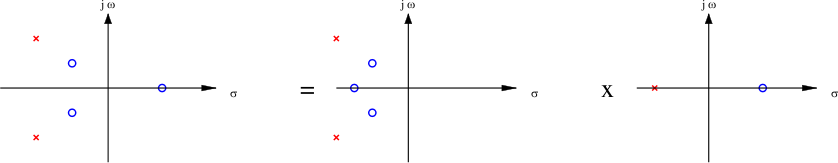
\includegraphics[width=12cm]{./bilder/nicht-minimalphasennetzwerk.png}\\
Nicht-Minimalphasennetzwerk (links) = Minimalphasennetzwerk (Mitte) · Allpass (rechts)

\subsection{Stabilitätsbestimmung am Pol-/Nullstellendiagramm}
\begin{tabular}{lcl}
	asymptotisch stabil & = & alle Polstellen in der linken Halbebene (LHE) \\
	grenzstabil			& = & Polstellen in der LHE und/oder auf der imaginären Achse
\end{tabular}

\subsection{Bode-Diagramm und Pol-Nullstellenverteilung von verschiedenen UTF
2. Ordnung}
Siehe \formelbuch{175}  

\subsection{Bode-Diagramm \matlab{bode}}
Siehe \formelbuch{178} für Beispiele\\
\begin{tabular}{ll}
	\parbox{7cm}{
		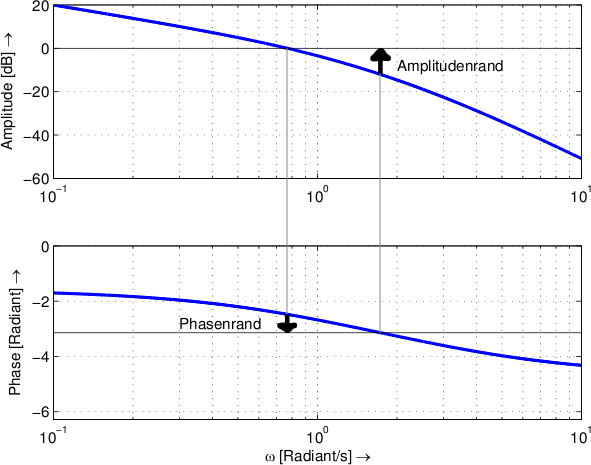
\includegraphics[width=7cm]{./bilder/bode-stabilitaet.png}
	}
	& \parbox{11cm}{
		\subsubsection{Definition}
		Das Bodediagramm besteht aus zwei Graphen, einer zeigt die Amplitude in
		doppelt-logarithmischer Form, der zweite zeigt die Phase in Grad und in
		linearer Form in Abhängigkeit der Frequenz dar.
		
		\subsubsection{Stabilitätsbestimmung \formelbuch{203} \matlab{margin,
		allmargin}}
		Der {\bf Amplitudenrand} ist der Abstand des
		Amplitudenganges zur 0~dB-Linie bei der Kreisfrequenz $\omega$, wo die Phase
		gleich $-\pi$ (-180 Grad) ist. \\
		
		Der {\bf Phasenrand} ist der Abstand das Phasenganges zur
		-$\pi$-Linie bei der Kreisfrequenz $\omega$, wo die Amplitude gleich 0~dB
		ist. \\
		
		Damit eine System stabil ist, m\"ussen Phasen- und Amplitudenrand
		$>0$ sein. Je gr\"osser der Phasen- und Amplitudenrand ist, desto
		``stabiler'' ist das System.
	}
\end{tabular}

\newpage 
\begin{landscape}
\subsection{Approximation des Bode-Diagramms}
\renewcommand{\arraystretch}{1.5}
\begin{longtable}{|l|l|ll|ll|}
	\hline
		\textbf{Pole} & 
		\textbf{UTF} $H(s)$ &
		\multicolumn{2}{c}{\textbf{Amplitude} $|H(s)|$} & 
		\multicolumn{2}{|c|}{\textbf{Phase} $\angle(H(s))$}
	\\ \hline
		Keine, konstanter Faktor &
		$\alpha e^{j \beta}$ &
		\parbox[c][1cm]{1cm}{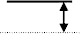
\includegraphics[width=1cm]{./bilder/bode-approx-konst.png}} &
		\, Konstant: $20 \log \alpha$ &
		\parbox[c][1cm]{1cm}{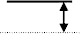
\includegraphics[width=1cm]{./bilder/bode-approx-konst.png}} &
		Konstant: $\beta$
	\\ \hline
		Pol im Ursprung &
		$\frac{\alpha}{s}$ &
		\parbox[c][1cm]{1cm}{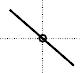
\includegraphics[width=1cm]{./bilder/bode-approx-ampl-tp-ord1.png}} & 
		\begin{tabular}{l}
			Lineare Steigung: $-20 dB/Dek.$ \\
			$0dB$ bei $\omega = \alpha$
		\end{tabular} &
		\parbox[c][1cm]{1cm}{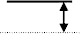
\includegraphics[width=1cm]{./bilder/bode-approx-konst.png}} & 
		Konstant: $-\frac{\pi}{2}$ 
	\\ \hline
		Nullstelle im Ursprung &
		$\alpha s$ &
		\parbox[c][1cm]{1cm}{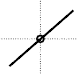
\includegraphics[width=1cm]{./bilder/bode-approx-ampl-hp-ord1.png}} & 
		\begin{tabular}{l}
			Lineare Steigung: $+20 dB/Dek.$ \\
			$0dB$ bei $\omega = \frac{1}{\alpha}$
		\end{tabular} &
		\parbox[c][1cm]{1cm}{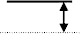
\includegraphics[width=1cm]{./bilder/bode-approx-konst.png}} &
		Konstant: $+\frac{\pi}{2}$
	\\ \hline	
		Reeller Pol &
		$\frac{1}{s + \alpha}$ &
		\parbox[c][1cm]{1cm}{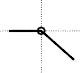
\includegraphics[width=1cm]{./bilder/bode-approx-ampl-4.png}} &
		\begin{tabular}{ll}
			$\omega < \alpha$: & Konstant $-20 \log \alpha$  \\
			$\omega > \alpha$: & $-20dB/Dek.$
		\end{tabular} &
		\parbox[c][1cm]{1cm}{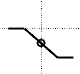
\includegraphics[width=1cm]{./bilder/bode-approx-phase-4.png}} &
		\begin{tabular}{ll}
			$\omega < \frac{\alpha}{10} $:	& Konstant $0$ \\
			$\omega > 10 \alpha$:		& Konstant $-\frac{\pi}{2}$
		\end{tabular}
	\\ \hline
		Reeller Pol &
		$\frac{\alpha}{s + \alpha}$ &
		\parbox[c][1cm]{1cm}{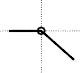
\includegraphics[width=1cm]{./bilder/bode-approx-ampl-4.png}} &
		\begin{tabular}{ll}
			$\omega < \alpha$: & Konstant $0dB$ \\
			$\omega > \alpha$: & $-20dB/Dek.$
		\end{tabular} &
		\parbox[c][1cm]{1cm}{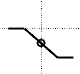
\includegraphics[width=1cm]{./bilder/bode-approx-phase-4.png}}	& 
		\begin{tabular}{ll}
			$\omega < \frac{\alpha}{10}$: & Konstant $0$ \\
			$\omega > 10 \alpha$: & Konstant $-\frac{\pi}{2}$
		\end{tabular}
	\\ \hline
		Reelle Nullstelle &
		$s + \alpha$ & 
		\parbox[c][1cm]{1cm}{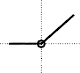
\includegraphics[width=1cm]{./bilder/bode-approx-ampl-5.png}} &
		\begin{tabular}{ll}
			$\omega < \alpha$: & Konstant $20 \log \alpha$ \\
			$\omega > \alpha$: & $+20dB/Dek.$
		\end{tabular} & 
		\parbox[c][1cm]{1cm}{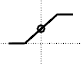
\includegraphics[width=1cm]{./bilder/bode-approx-phase-5.png}}	&
		\begin{tabular}{ll}
			$\omega < \frac{\alpha}{10}$: & Konstant $0$ \\
			$\omega > 10 \alpha$: & Konstant $+\frac{\pi}{2}$
		\end{tabular}
	\\ \hline	
		Reelle Nullstelle &
		$\frac{s + \alpha}{\alpha}$ &
		\parbox[c][1cm]{1cm}{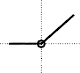
\includegraphics[width=1cm]{./bilder/bode-approx-ampl-5.png}} &
		\begin{tabular}{ll}
			$\omega < \alpha$: & Konstant $0dB$ \\
			$\omega > \alpha$: & $+20dB/Dek.$
		\end{tabular} &
		\parbox[c][1cm]{1cm}{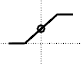
\includegraphics[width=1cm]{./bilder/bode-approx-phase-5.png}} &
		\begin{tabular}{ll}
			$\omega < \frac{\alpha}{10}$: & Konstant $0$ \\
			$\omega > 10 \alpha$: & Konstant $+\frac{\pi}{2}$
		\end{tabular}
	\\ \hline
		Konjugiert-komplexe Pole &
		$\frac{1}{s^2+s\frac{\omega_p}{q_p}+\omega_p^2}$ &
		\parbox[c][1cm]{1cm}{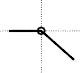
\includegraphics[width=1cm]{./bilder/bode-approx-ampl-6.png}} &
		\begin{tabular}{ll}
			$\omega < \omega_p$: 	& Konstant $-40 \log \omega_p$ \\
			$\omega > \omega_p$:	& $-40dB/Dek.$ \\
			Überhöhung: 			& $\frac{\omega_p}{2}$ bis $2\omega_p$ \\
			Maximum:				& $20 \log q_p$ bei $\omega = \omega_p$			
		\end{tabular} &
		\parbox[c][1cm]{1cm}{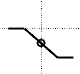
\includegraphics[width=1cm]{./bilder/bode-approx-phase-6.png}} &
		\begin{tabular}{ll}
			$\omega < \frac{\omega_p}{10^{\frac{1}{2q_p}}}$:	& Konstant $0$ \\
			$\omega > \omega_p 10^{\frac{1}{2q_p}}$:			& Konstant $-\pi$ \\
			$\omega = \omega_p$:								& $-\frac{\pi}{2}$
		\end{tabular}
	\\ \hline
		Konjugiert-komplexe Pole &
		$\frac{\omega_p^2}{s^2+s\frac{\omega_p}{q_p}+\omega_p^2}$ & 
		\parbox[c][1cm]{1cm}{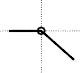
\includegraphics[width=1cm]{./bilder/bode-approx-ampl-6.png}} &
		\begin{tabular}{ll}
			$\omega < \omega_p$:	& Konstant $0dB$ \\
			$\omega > \omega_p$:	& $-40dB/Dek.$ \\
			Überhöhung:				& $\frac{\omega_p}{2}$ bis $2 \omega_p$ \\
			Maximum:				& $20 \log q_p$ bei $\omega = \omega_p$
		\end{tabular} &
		\parbox[c][1cm]{1cm}{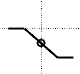
\includegraphics[width=1cm]{./bilder/bode-approx-phase-6.png}}	& 
		\begin{tabular}{ll}
			$\omega < \frac{\omega_p}{10^{\frac{1}{2q_p}}}$:	& Konstant $0$ \\
			$\omega > \omega_p 10^{\frac{1}{2q_p}}$:			& Konstant $-\pi$ \\
			$\omega = \omega_p$:								& $-\frac{\pi}{2}$
		\end{tabular}
	\\ \hline	
		Konjugiert-komplexe Nullstellen &
		$s^2+s\frac{\omega_z}{q_z}+\omega_z^2$ &
		\multicolumn{4}{l|}{
			Analog zu den Konjugiert-komplexen Polen jedoch gespiegelt an der $0dB$- / $0$-Grad-Linie.
		}
	\\
		&
		$\frac{s^2+s\frac{\omega_z}{q_z}+\omega_z^2}{\omega_z^2}$ &
		\multicolumn{4}{l|}{}
	\\ \hline
		\multicolumn{6}{|p{21cm}|}{
			Serieschaltung von Systemen erfolgt durch \textbf{Superposition} der einzelnen Bode-Diagramme 
			(Multiplikation von UTFs entspricht Addition im	dB-Bereich).
		}
	\\ \hline
\end{longtable}
\renewcommand{\arraystretch}{\arraystretchOriginal}
\end{landscape}
\renewcommand{\arraystretch}{1}

\textbf{Werte für $q_p$ bzw. $q_z$}\\
\renewcommand{\arraystretch}{1.5}
\begin{tabular}{|r|r|r||r|r|r||r|r|r||r|r|r||r|r|r|}
\hline
\multicolumn{1}{|l|}{$q$} & \multicolumn{1}{l|}{$10^{\frac{1}{2 q_p}}$} & 
\multicolumn{1}{l||}{$\frac{1}{10^{\frac{1}{2 q_p}}}$} &
\multicolumn{1}{l|}{$q$} & \multicolumn{1}{l|}{$10^{\frac{1}{2 q_p}}$} &
\multicolumn{1}{l||}{$\frac{1}{10^{\frac{1}{2 q_p}}}$} &
\multicolumn{1}{l|}{$q$} & \multicolumn{1}{l|}{$10^{\frac{1}{2 q_p}}$} & \multicolumn{1}{l||}{$\frac{1}{10^{\frac{1}{2 q_p}}}$} & \multicolumn{1}{l|}{$q$} & \multicolumn{1}{l|}{$10^{\frac{1}{2 q_p}}$} & \multicolumn{1}{l||}{$\frac{1}{10^{\frac{1}{2 q_p}}}$} & \multicolumn{1}{l|}{$q$} & \multicolumn{1}{l|}{$10^{\frac{1}{2 q_p}}$} & \multicolumn{1}{l|}{$\frac{1}{10^{\frac{1}{2 q_p}}}$} \\ \hline
\hline
1 & 3.162 & 0.316 & 5 & 1.259 & 0.794 & 9 & 1.136 & 0.880 & 13 & 1.093 & 0.915 & 17 & 1.070 & 0.935 \\ \hline
2 & 1.778 & 0.562 & 6 & 1.212 & 0.825 & 10 & 1.122 & 0.891 & 14 & 1.086 & 0.921 & 18 & 1.066 & 0.938 \\ \hline
3 & 1.468 & 0.681 & 7 & 1.179 & 0.848 & 11 & 1.110 & 0.901 & 15 & 1.080 & 0.926 & 19 & 1.062 & 0.941 \\ \hline
4 & 1.334 & 0.750 & 8 & 1.155 & 0.866 & 12 & 1.101 & 0.909 & 16 & 1.075 & 0.931 & 20 & 1.059 & 0.944 \\ \hline
\end{tabular}
\renewcommand{\arraystretch}{1}\\


\subsection{Ortskurve (Nyquist-Diagramm) \formelbuch{198} \matlab{nyquist}}
\begin{tabular}{ll}
	\parbox{7cm}{
		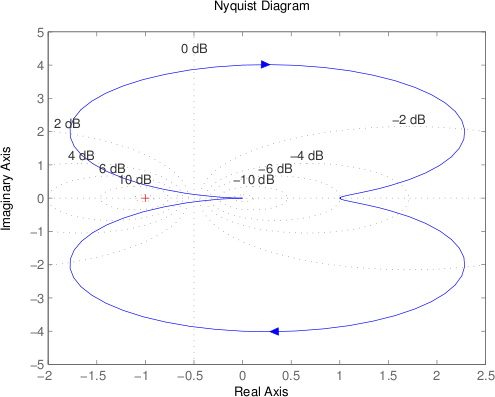
\includegraphics[width=7cm]{./bilder/nyquist.png}
	}
	& \parbox{11cm}{
		\subsubsection{Definition}
		Im Gegensatz zum Bode-Diagramm wird beim Nyquist-Diagramm Betrag und Phase in
		einem einzigen Diagramm dargestellt, nämlich indem man den Real- und
		Imaginärteil des Ausgabewertes direkt in die komplexe Zahlenebene zeichnet.
		
		\subsubsection{Stabilitätsbestimmung}
		Ist der {\bf offene} Regelkreis $H(s)$ {\bf asymptotisch
		stabil}\index{asymptotisch stabil}, so ist der {\bf geschlossene}
		Regelkreis $1+H(s)=D(s)+N(s)$ asymptotisch stabil, wenn die {\bf
		Ortskurve} des {\bf offenen} Regelkreises den kritischen Punkt
		(-1,$j0$) weder umkreist noch durchl\"auft.
	}
\end{tabular}


\subsection{Nichols-Diagramm \formelbuch{203} \matlab{nichols}}
\begin{tabular}{ll}
	\parbox{7cm}{
		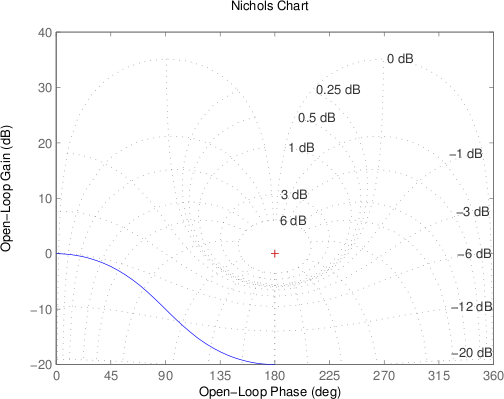
\includegraphics[width=7cm]{./bilder/nichols.png}
	}
	& \parbox{11cm}{
		\subsubsection{Definition}
		Das Nichols Diagramm (auch Amplituden-Phasen-Diagramm) ist die Darstellung des
		Absolutbetrages (Verstärkung, logarithmisch) in Abhängigkeit der Phase. Das Nichols Diagramm ist zur
		Bestimmung der Stabilität in rückgekoppelten Systemen verwendbar.
	}
\end{tabular}

\newpage

\section{Signalflussdiagramm \formelbuch{213}}
\begin{list}{$\bullet$}{\setlength{\itemsep}{0cm} \setlength{\parsep}{0cm} \setlength{\topsep}{0cm}} 
  \item Graphische Lösung linearer Gleichungen
  \item Graphische Darstellung von LTI-Systemen
  \item Änderung der Topologie ohne UTF zu ändern
\end{list}

\subsection{Glossar \formelbuch{213}}
  \begin{tabular}{|m{4cm} | m{14cm}|}
    \hline
      \textbf{Knoten}: &
      Darstellung einer Grösse, eines Signals oder einer Variable \\
    \hline
      \textbf{Zweig}: &
      Funktionelle Abhängigkeit einer Grösse \\
    \hline
      \textbf{Quelle}: &
      Unabhängiger Knoten, es münden keine Zweige ein \\
    \hline
      \textbf{Senke}: &
      Knoten, ohne weggehende Zweige \\
    \hline
      \textbf{Pfad}: &
      Kontinuierliche Folge von Zweigen, die in die gleiche Richtung zeigen \\
    \hline
      \textbf{Offener Pfade}: &
      Ein Pfad, bei dem jeder beteiligte Knoten nur einmal durchquert wird \\
      \textbf{Vorwärtspfad}: &
      Ein offener Pfad zwischen einer Quelle und einer Senke \\
    \hline
      \textbf{Schleife}: &
      Ein geschlossener Pfad, welcher zum Ausgangsknoten zurückkehrt, 
      wobei jeder beteiligte Knoten nur einmal durchlaufen wird, ausgenommen der
      Ausgangsknoten \\
    \hline
      \textbf{Eigenschleife}: &
      Eine (Rückkopplungs)schleife, die aus einem Zweig und einem Knoten besteht \\
    \hline
      \textbf{Zweigtransmittanz}: &
      Die lineare Grösse, unabhängig von ihrer Dimension, 
      die einen Knoten eines Zweiges zum anderen Knoten in Beziehung setzt. \\
    \hline
      \textbf{Schleifentransmittanz}: &
      Das Produkt der Zweigtransmittanzen in einer Schleife. \\
    \hline
  \end{tabular}

\subsection{Transformationsregeln \formelbuch{219ff.}}
  \begin{multicols}{2}
    \subsubsection{Transmittanzverschiebung\formelbuch{220}}
      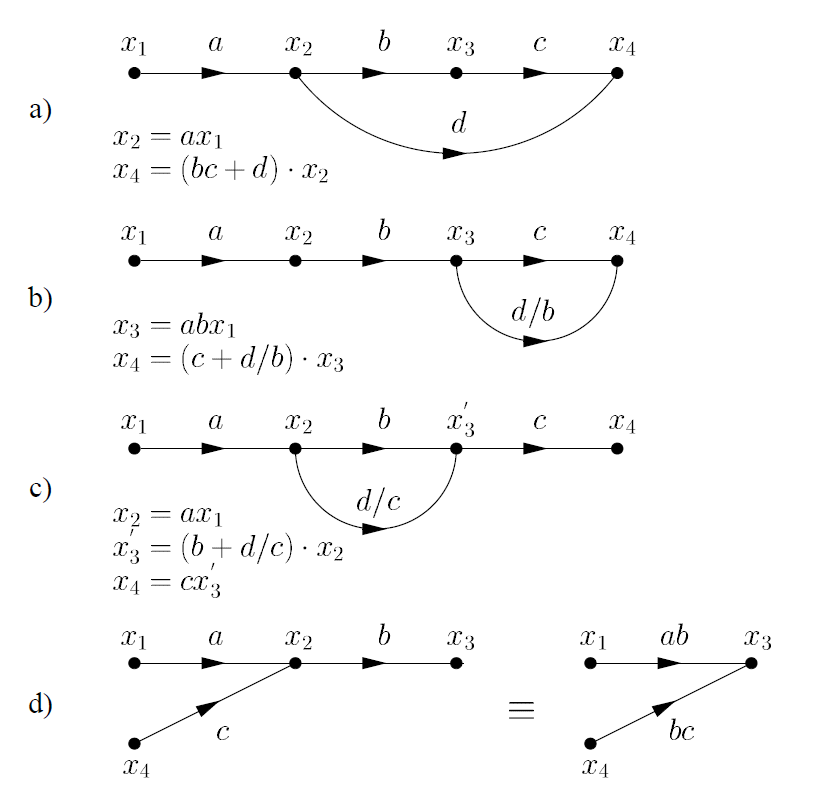
\includegraphics[width=7cm]{./images/transmittanzverschiebung.png} \\
      Wichtig ist, dass eine neue Variable eingeführt wird, wenn wenn der Endpunkt eines
      inneren Zweiges verschoben wird. (siehe c)
      \vfill
  \columnbreak
  
    \subsubsection{Pfadinversion\formelbuch{221}}
      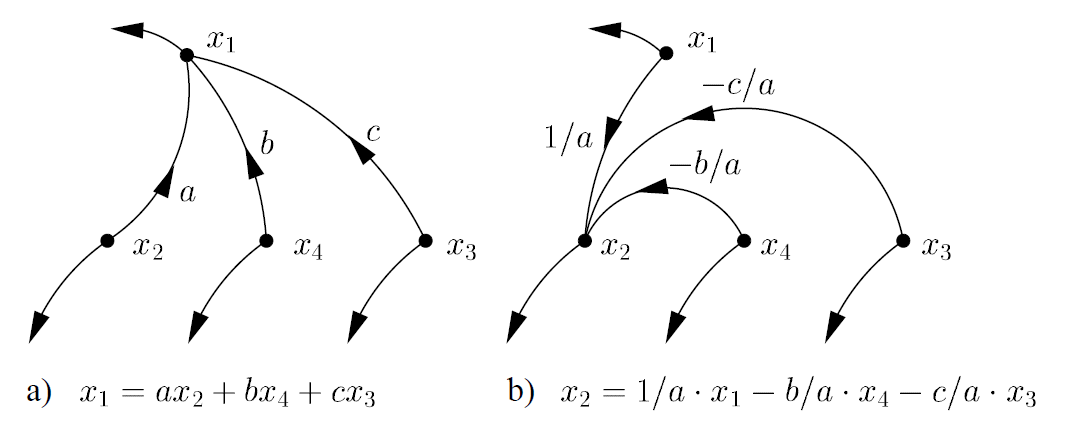
\includegraphics[width=8cm]{./images/pfadinversion.png} \\
      Es gilt zu beachten, das die Inversion eines Pfaden (dessen Anfangspunkt nach Definition
      eine Quelle sein muss) den Effekt hat, dass die Quelle vom einen Ende des Pfades zum anderen
      Ende verschoben wird. Der Pfad von $x_i$ nach $x_j$ hat eine Transmittanz von $L$. 
      Den zu invertierenden Pfad setzten wir $\frac{1}{L}$ und alle Pfade welche ursprünglich in
      $x_i$ endeten, werden verschoben, dass sie neu in $x_j$ enden und ihre Transmittanzen werden
      mit $-\frac{1}{L}$ multipliziert.
      
    \subsubsection{Entfernen einer Eigenschleife\formelbuch{222}}
      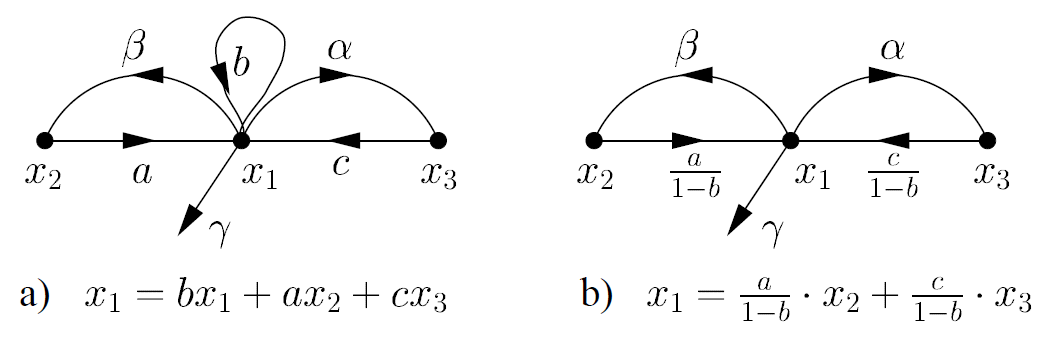
\includegraphics[width=8cm]{./images/eigenschleife.png} \\
      Die Eigenschleife hat die Transmittanz $L$. Sie wird entfernt indem man bei allen anderen
      Zweigen welche \textbf{in den Knoten münden}, durch $(1-L)$ \textbf{dividiert}.
 \end{multicols}
 
\newpage 

\subsection{Mason's Regel \formelbuch{227}}
  $\boxed{H_{ij} = \frac{\sum\limits_k P_k\cdot\Delta_k}{\Delta}}\quad
  \Rightarrow$ UTF von $x_i$ nach $x_j$, wobei \textbf{$x_i$} eine
  \textbf{Quelle}, \textbf{$x_j$} jedoch nicht zwingend eine \textbf{Senke} sein
  muss. \vspace{0.3cm}\\
  $P_k \Rightarrow$ Vorwärtspfad $k$ (bezogen auf 1 Eingang) \qquad $\Delta_k \Rightarrow$ Kofaktor de
  $k$-ten Pfades \qquad $\Delta \Rightarrow$ Netzwerkdet/Graphdet\vspace{0.3cm}\\
  $\Delta$ = 1- (Summe aller Schleifen) + (Summe aller Produkte zweier
  Schleifen, die sich nicht berühren) - (Summe
  aller Produkte dreier Schleifen, die sich nicht berühren) + $\ldots$
  \vspace{0.3cm}\\
  $\Delta_k$ = 1- (Summe aller Schleifen die $P_k$ nicht berühren) + (Summe
  aller Produkte zweier Schleifen, die $P_k$ und sich selbst nicht
  berühren)-(Summe aller Produkte dreier Schleifen, die $P_k$ und sich selbst
  nicht berühren) + $\ldots$ \\

  Falls die \textbf{UTF eines SFD von einem beliebigen Knoten} (keiner Quelle)
  gesucht wird, kann Mason's Regel nicht direkt angewandt werden. Abhilfe: \\
  $\boxed{H_{ij} = \frac{x_j}{x_i} = \frac{x_j}{x_q} \frac{x_q}{x_i} =
  \frac{H_{qj}}{H_{qi}}}$ Wobei $x_q$ eine Quelle sei. 
  Schlussendlich kürzt sich die Netzwerkdeterminante heraus.


\subsection{Beispiel eines SFD \formelbuch{231}}
\begin{tabular}{ll}
	\parbox{7cm}{
    	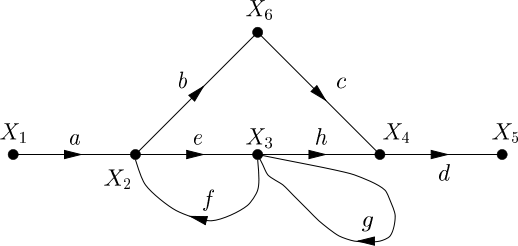
\includegraphics[width=7cm]{./images/sfd-bsp.png}
    }
    
    & \parbox{12cm}{
    \begin{enumerate}
		\item[a)] Die UTF\index{UTF} zwischen $X_1$ und $X_4$ ist (mit Mason's Regel):\index{Mason's Regel}\\
		\begin{equation*}
		H_{14}=\frac{X_4}{X_1}=\frac{aeh+abc(1-g)}{1-ef-g}
		\end{equation*}
		\item[b)] Das folgende Gleichungssystem beschreibt das SFD.
		\begin{eqnarray*}
		X_2 &=&a\cdot X_1+f\cdot X_3\\
		X_3 &=&e\cdot X_2+g\cdot X_3\\
		X_4 &=&h\cdot X_3+c\cdot X_6\\
		X_5 &=&d\cdot X_4\\
		X_6 &=&b\cdot X_2
		\end{eqnarray*}
		Nach Umformung der Gleichungen erhalten wir:
		\begin{equation*}
		X_4=h\cdot X_3+\frac{bc}{e}\cdot (1-g)\cdot X_3\quad\&\quad X_3\cdot
		\frac{1-g}{e}=a\cdot X_1+f\cdot X3.
		\end{equation*}
		Somit ist $X_4=\frac{h+\frac{bc}{e}(1-g)}{\frac{1-g}{ae}-\frac{f}{a}}X_1=\frac{aeh+abc(1-g)}{1-g-ef}X_1$.
	\end{enumerate}}
\end{tabular}

\subsection{Fundamentales SFD \formelbuch{232}}
\begin{tabular}{ll}
	\parbox{7cm}{
    	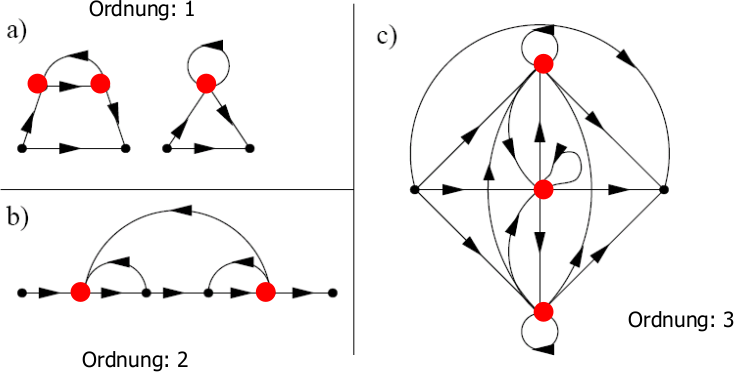
\includegraphics[width=7cm]{./images/sfd-ordnung.png}
    }
    
    & \parbox{12cm}{
		\textit{Ordnung eines SFD = Anzahl der fundamentalen Knoten}: Knoten, welche
		entfernt werden müssen, um \textit{alle} Schleifen aufzubrechen. \\ \\
	}
\end{tabular}

\subsubsection{Fundamentales SFD erster Ordnung \formelbuch{233}}
\begin{tabular}{ll}
	\parbox{7cm}{
    	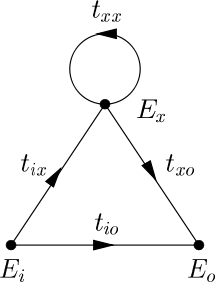
\includegraphics[width=3cm]{./images/sfd-fundamental-erster-ordnung.png}
    }
    & \parbox{12cm}{
		Durch Reduzieren auf das fundamentale SFD 1. Ordnung, kann die UTF direkt
		ermittelt werden: \\
		\[ H_{io} = \frac{E_o}{E_i}=
		t_{io}+\frac{t_{ix}t_{xo}}{1-t_{xx}}=
		\frac{t_{io}-t_{io}t_{xx}+t_{ix}t_{xo}}{1-t_{xx}} \] \\
    \begin{tabular}{l l p{8cm}}
      $E_x$ & = & Fundamentaler Knoten\\
      $E_i$ & = & Quelle (Eingang) \\
      $E_o$ & = & Senke (Ausgang) \\
      $t_{xx}$ & = & alle Eigenschleifen des Knoten $E_x$ \\
      $t_{ix}$ & = & alle Pfade von der Quelle zum Knoten $E_x$ \\
      $t_{xo}$ & = &alle Pfade vom Knoten $E_x$ zur Senke \\
      $t_{io}$ & = & Leckpfad, alle Pfade von der Quelle zur Senke, welche \underline{nicht}
      durch den Knoten $E_x$ führen.
    \end{tabular}\\
    Wenn es mehrere Wege gibt, dann zusammen zählen: Bsp.: $tix = tix_1 +
    tix_2$
	}
\end{tabular}


\subsection{Einbezug analoger Verstärker \formelbuch{238}}
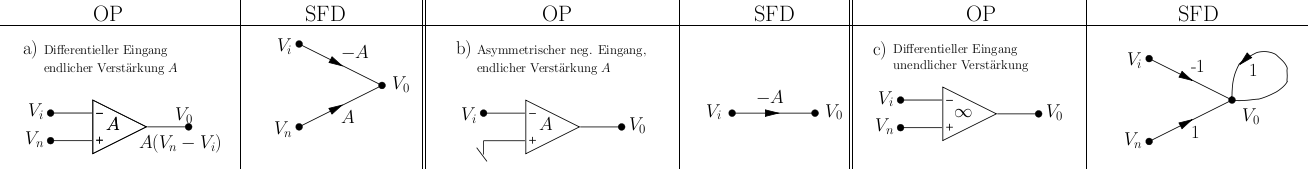
\includegraphics[width=18cm]{./images/sfd-op.png}

\subsection{Skalierung\formelbuch{243}}
	Um einen oder mehrere Knoten zu ändern, ohne das gesamte System zu
	ändern (Voraussetzung: Start/Endknoten werden nicht mitmaskiert), kann man
	diese Knoten skalieren.\\
	Vorgehen: 
	\begin{enumerate}
                \item Skalierungszone festlegen (Trennbündel) $N_b$
                \item Alle eingehende Zweige mit $\lambda$ multiplizieren
                \item Alle ausgehende Zweige mit $\frac{1}{\lambda}$
                multiplizieren
    \end{enumerate}
    Wenn alle maximalen Signalniveaus gleich $\rightarrow$ maximal möglichen
    Dynamikbereich\\
    \begin{minipage}{9cm}
      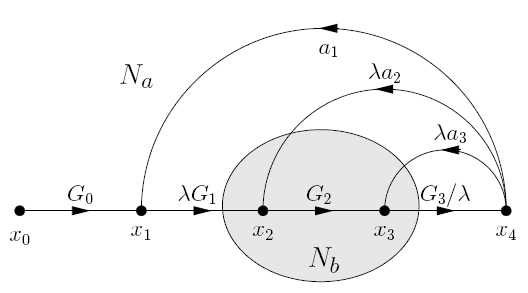
\includegraphics[width=7cm]{./images/sfd-scalierung.png}
    \end{minipage}
    \begin{minipage}{9cm}
      Die Skalierung kann verwendet werden um den Dynamikbereich zu maximieren, Inverter zu entfernen
      und die Verstärkung und Signalniveaus innerhalb eines Systems zu ändern.
    \end{minipage}
    
\subsection{Transposition\formelbuch{242}}
  \begin{multicols}{2}
    \textbf{Ablauf:}
    \begin{enumerate}
      \item Richtungsumdrehung aller Zweigtransmittanzen bei gleichbleibenden Transmittanzen
      \item Spiegelung des resultierenden SFD
      \item Bezeichnungswechsel von Eingangs- und Ausgangsknoten
    \end{enumerate}
    
    Die UTF des transponierten SFD ist \textbf{identisch} mit der UTF des ursprünglichen SFD, aber ihre
    Topologie ist verschieden.
    
  \columnbreak
    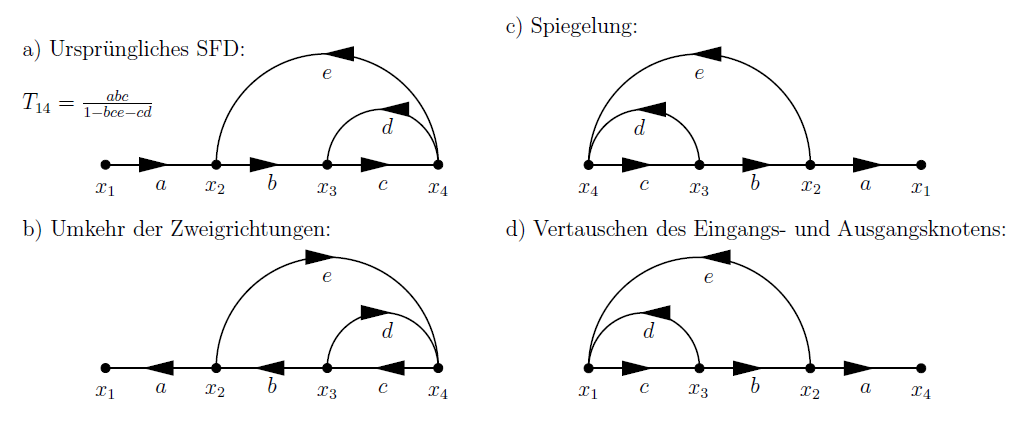
\includegraphics[width=9cm]{./images/transposition.png}
  \end{multicols}
    


\newpage

\section{Zustandsraumdarstellung (ZRD)\formelbuch{265}}
Darstellung einer Differentialgleichung $n$. Ordnung durch ein
Differentialgleichungssystem von $n$ Gleichungen 1. Ordnung.

\subsection{Definition \formelbuch{267}}
\begin{multicols}{2}
	\adjustbox{width=\linewidth}{\begin{tikzpicture}
%Names
\node at (0,0) [anchor=east] {$\underline{u}(t)$};
\node at (2.5,0.1) [anchor=south] {$\dot{x}(t)$};
\node at (4.5,0.1) [anchor=south] {$x(t)$};
\node at (7,0) [anchor=west] {$\underline{y}(t)$};

%Boxes
\draw (1,0.5) rectangle (2,-0.5);
\node at (1.5,0) {B};
\draw (3,0.5) rectangle (4,-0.5);
\node at (3.5,0) {$\frac{1}{s}$};
\draw (3,1) rectangle (4,2);
\node at (3.5,1.5) {D};
\draw (3,-1) rectangle (4,-2);
\node at (3.5,-1.5) {A};
\draw (5,0.5) rectangle (6,-0.5);
\node at (5.5,0) {C};

%Operators
\draw (2.5,0) circle (0.15);
\draw (2.4,0) -- (2.6,0);
\draw (2.5,-0.1) -- (2.5,0.1);

\draw (6.5,0) circle (0.15);
\draw (6.4,0) -- (6.6,0);
\draw (6.5,-0.1) -- (6.5,0.1);

%Arrows
%Middle
\draw [->] (0,0) -- (1,0);
\draw [->] (2,0) -- (2.35,0);
\draw [->] (2.65,0) -- (3,0);
\draw [->] (4,0) -- (5,0);
\draw [->] (6,0) -- (6.35,0);
\draw [->] (6.65,0) -- (7,0);
%Top
\draw [->] (0.5,0) -- (0.5,1.5) -- (3,1.5);
\draw [->] (4,1.5) -- (6.5,1.5) -- (6.5,0.15);
%Bottom
\draw [->] (4.5,0) -- (4.5,-1.5) -- (4,-1.5);
\draw [->] (3,-1.5) -- (2.5,-1.5) -- (2.5,-0.15);


\end{tikzpicture}}
	
	Bestimmung der Matrizen A,B,C,D siehe auch \formelbuch{298}
	
	$\dot{\underline{x}}(t) = {\boldsymbol A} \underline{x}(t) + {\boldsymbol B} \underline{u}(t)$ 
  \qquad (Zustandsgleichung) \\
	$\underline{y}(t) = {\boldsymbol C} \underline{x}(t) + {\boldsymbol D} \underline{u}(t)$ \qquad (Ausgangsgleichung)
		
	\begin{description}[noitemsep, style=multiline, leftmargin=15pt]
  		\item[A] Systemmatrix ($n$ x $n$)
  		\item[B] Steuer- oder Eingangsmatrix ($n$ x $m$) ``senkrecht''
  		\item[C] Beobachtungs- oder Ausgangsmatrix ($k$ x $n$) ``waagrecht''
  		\item[D] Übergangs- oder Durchgangsmatrix ($k$ x $m$) \\
  		\item[m] Anzahl Eingänge
  		\item[n] Anzahl Integratoren (Ordnung)
  		\item[k] Anzahl Ausgänge
	\end{description}	
\end{multicols}

\subsection{Äquivalente ZRD\formelbuch{269}}
  \begin{tabular}{p{6cm}p{6cm}p{6cm}}
    \[\underline{\dot{\xi}}(t) = \underbrace{\mathbf{TAT^{-1}}}_{\hat A}\underline\xi(t) +
    \underbrace{\mathbf{TB}}_{\hat B}\underline u(t) \] &
    
    \[ \underline y(t) = \underbrace{\mathbf{CT^{-1}}}_{\hat C}\underline\xi(t) +
    \underbrace{D}_{\hat D}\underline u(t) \] &
    
    $\mathbf{T}$: Transformationsmatrix mit \newline
    $\mathbf{TT^{-1}=T^{-1}T=I}$ \newline
    Mit der Transformationsmatrix kann man verschiedenste Zustandgrössen und ZRD erhalten,
    die aber alle ein identisches Systemverhalten aufweisen.
  \end{tabular}
  
\subsection{Stabilität \formelbuch{285}}
  Wenn alle Realteile der Eigenwerte $\lambda$ der Systemmatrix ${\boldsymbol A}$
  negativ sind, ist ein LTI-System asymptotisch stabil, \newline
  $\left | \lambda\boldsymbol{I} - \boldsymbol{A} \right |   =0 \rightarrow \forall~\lambda \quad\Re \{\lambda\}<0$
  jedoch nicht umgekehrt. 

\subsection{ZRD im Zeitbereich \formelbuch{270}}

\subsection{ZRD im Frequenzbereich \formelbuch{274} \matlab{ss2tf}}
  \[ \boldsymbol{H(s)} = \frac{\underline{Y}(s)}{\underline{U}(s)} =
  \boldsymbol{C}\left(s\boldsymbol{I}-\boldsymbol{A}\right)^{-1}\boldsymbol{B}+\boldsymbol{D} \qquad
   (\text{Anfangsbedingungen: } \vec{x(0)} = \vec 0) \]
  \\
  Die Grösse der Matrix $\boldsymbol {H(s)}$ entspricht der Grösse der
  Durchgangsmatrix $\boldsymbol D$. $\boldsymbol{I}$ sei die Einheitsmatrix mit
  Grösse $n$ x $n$.
  
  \begin{align*}
    H(s) &= \left[
    \begin{array}{c c}
      C_{11}  & C_{12}\\
    \end{array}
    \right] \cdot \left( \left[
    \begin{array}{cc}
      s & 0\\
      0 & s\\
    \end{array}
    \right] - \left[
    \begin{array}{cc}
      A_{11} & A_{12}\\
      A_{21} & A_{22}\\
    \end{array}
    \right] \right)^{-1} \cdot \left[
    \begin{array}{c}
      B_{11}\\
      B_{21}\\
    \end{array}
    \right ]+ D \\
    &=  \frac{B_{11}C_{11}(s-A_{22}) + B_{11}C_{12}A_{21} + B_{21}C_{11}A_{12} + B_{21}C_{12}(s-A_{11})}
		{(s-A_{22})(s-A_{11}) - A_{12}A_{21}} + D
  \end{align*}

  Ist die Übertragungsfunktion $H_{ba}(s)$ vom \textbf{Eingang b} zum \textbf{Ausgang a} gesucht, so gilt:
  \[
    H_{ba}(s) = \frac{Y_a(s)}{U_b(s)} = C(a,:) \cdot (s \cdot I -A)^{-1} \cdot B(:,b) + D(a,b)
  \]

\newpage

\subsection{Bestimmung der ZRD aus der UTF\formelbuch{277}}
  \[ \boxed{
  H(s)=\frac{Y(s)}{U(s)}=\frac{b_{m} s^{m} + b_{m-1} s^{m-1} +\cdots+b_{1} s 
  + b_{0}}{s^{n} + a_{n-1} s^{n-1} + \cdots + a_{1} s + a_{0}}}
  \]\\
  Allgemeine Formel für $m=1$ Eingang, $k=1$ Ausgang, $n=2$ Integratoren:


\subsubsection{Regelungsnormalform \formelbuch{277}}
  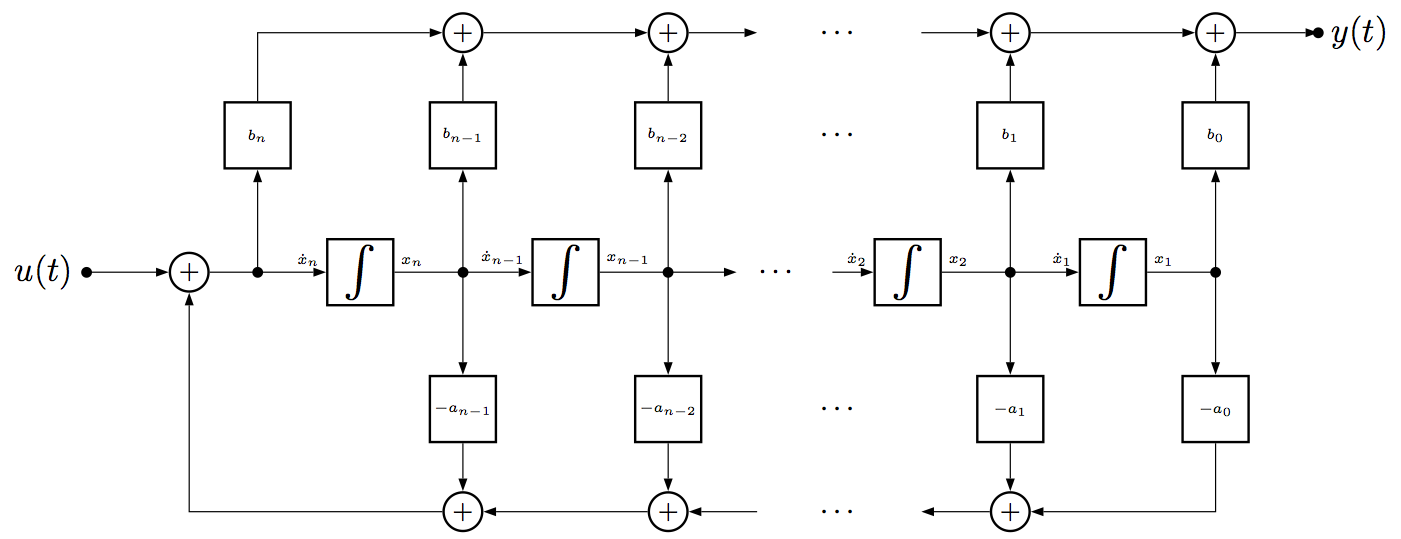
\includegraphics[width=10cm]{./images/zrd-regelungsnormalform.png} \\
  \scriptsize
  \begin{equation*}
    \left [ 
    \begin{array}{c}
      \dot{x}_1(t)\\
      \dot{x}_2(t)\\
      \vdots\\
      \dot{x}_{n-1}(t)\\
      \dot{x}_{n}(t)\\
    \end{array}
    \right ] =
    \left [ 
    \begin{array}{c c c c c}
      0 & 1 & 0 & \ldots & 0\\
      0 & 0 & 1 & \ldots & 0\\
      \vdots & \vdots & \vdots & \ddots & \vdots\\
      0 & 0 & 0 & \ldots & 1\\
      -a_0 & -a_1 & -a_2 & \ldots & -a_{n-1}\\
    \end{array}
    \right ]\cdot
    \left [ 
    \begin{array}{c}
      x_1(t)\\
      x_2(t)\\
      \vdots \\
      x_{n-1}(t)\\
      x_{n}(t)\\
    \end{array}
    \right ]+
    \left [ 
    \begin{array}{c}
      0 \\
      0\\
      \vdots\\
      0\\
      1\\
    \end{array}
    \right ]\cdot
    u(t),
  \end{equation*}
  \begin{equation*}
    y(t) = 
    \left [ 
    \begin{array}{c c c c}
      b_0-a_0b_n & b_1-a_1b_n & \ldots & b_{n-1}-a_{n-1}b_n\\
    \end{array}
    \right ] \cdot
    \left [ 
    \begin{array}{c}
      x_1(t)\\
      x_2(t)\\
      \vdots \\
      x_{n-1}(t)\\
      x_{n}(t)\\
    \end{array}
    \right ]+
    \left [ 
    \begin{array}{c}
      b_n \\
    \end{array}
    \right ] \cdot
    u(t).
  \end{equation*}
  \normalsize

\begin{samepage}
\subsubsection{Beobachtungsnormalform \formelbuch{279 }}
  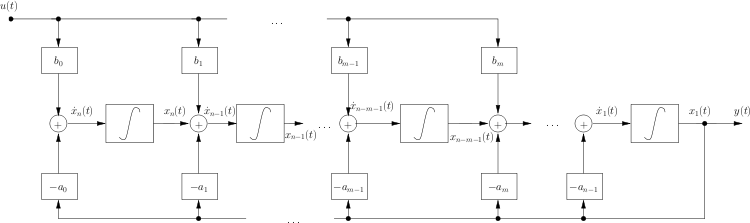
\includegraphics[width=10cm]{./images/zrd-beobachtungsnormalform.png} \\
  \scriptsize
  \begin{eqnarray*}
    \left [ 
    \begin{array}{c}
      \dot{x}_1(t)\\
      \dot{x}_2(t)\\
      \vdots\\
      \dot{x}_{n-1}(t)\\
      \dot{x}_n(t)\\
    \end{array}
    \right ] &=&
    \left [ 
    \begin{array}{c c c c c}
      0 & 0 & 0 & \ldots & -a_0\\
      1 & 0 & 0 & \ldots & -a_1\\
      0 & 1 & 0 & \ldots & -a_2\\
      \vdots & \vdots &  \ddots & 0 & \vdots\\
      0 & 0 & \ldots & 1 & -a_{n-1}\\
    \end{array}
    \right ]\cdot
    \left [ 
    \begin{array}{c}
      x_1(t)\\
      x_2(t)\\
      \vdots \\
      x_{n-1}(t)\\
      x_{n}(t)\\
    \end{array}
    \right ]+
    \left [ 
    \begin{array}{c}
      b_0-a_0b_n \\
      b_1-a_1b_n\\
      b_2-a_2b_n\\
      \vdots\\
      b_{n-1}-a_{n-1}b_n\\
    \end{array}
    \right ]\cdot
    u(t),\\
    y(t) &= &
    \left [ 
    \begin{array}{c c c c}
      0 & 0 & \ldots & 1\\
    \end{array}
    \right ] \cdot
    \left [ 
    \begin{array}{c}
      x_1(t)\\
      x_2(t)\\
      \vdots \\
      x_{n-1}(t)\\
      x_{n}(t)\\
    \end{array}
    \right ]+
    \left [ 
    \begin{array}{c}
      b_n \\
    \end{array}
    \right ] \cdot
    u(t).
  \end{eqnarray*}
  \normalsize
\end{samepage}

\newpage

\begin{multicols}{2}
\subsubsection{Digaonalform\formelbuch{281}}
  Für einfache, reelle Pole mit $m=n$ \\
  \scriptsize
    
    \begin{eqnarray*}
      \begin{bmatrix}
        \dot{x}_1(t) \\
        \dot{x}_2(t) \\
        \vdots \\
        \dot{x}_{n-1}(t) \\
        \dot{x}_n(t)
      \end{bmatrix} &=& \overbrace{ \begin{bmatrix}
        p_1 & 0 & 0 & \ldots & 0 \\
        0 & p_2 & 0 & \ldots & 0 \\
        0 & 0 & p_3 & \ldots & 0 \\
        \vdots & \vdots & \ddots & p_{n-1} & \vdots \\
        0 & 0 & \ldots & 0 & p_n
      \end{bmatrix}}^{\mathbf A} \cdot \begin{bmatrix}
        x_1(t) \\
        x_1(t) \\
        \vdots \\
        x_{n-1}(t) \\
        x_n(t)
      \end{bmatrix} + \overbrace{\begin{bmatrix}
        1 \\
        1 \\
        1 \\
        \vdots \\
        1 \\
      \end{bmatrix}}^{\mathbf{B}} \cdot u(t) \\
      y(t) &=& \overbrace{\begin{bmatrix}
        \alpha_1 & \alpha_2 & \ldots & \alpha_n
      \end{bmatrix}}^{\mathbf{C}} \cdot \begin{bmatrix}
        x_1(t) \\
        x_1(t) \\
        \vdots \\
        x_{n-1}(t) \\
        x_n(t)
      \end{bmatrix} + \overbrace{[b_n]}^{\mathbf{D}} \cdot u(t)
    \end{eqnarray*}
  \normalsize

\columnbreak

\subsubsection{Jordan-Normalform\formelbuch{283}}
  Ist für mehrfache, reelle Pole. Die Jordan-Normalform ist gleich aufgebaut wie die Diagonalform, 
  es kann jedoch auf der oberen Nebendiagonalen z.T 1 haben. \\
  Mehr Details im Skript S.283
\end{multicols}


\subsection{Beobachtbar- \& Steuerbarkeit \formelbuch{287}}
\subsubsection{Steuerbarkeit\formelbuch{287} \matlab{ctrb}}
Gibt es Zustände von $\underline{x} (t)$ die nicht von den
Eingängen $\underline{u} (t)$ beeinflusst werden? Wenn ja,
dann ist das System nicht steuerbar!

Wenn $|Q_{Steuerbarkeit}|= \left| \left [ \boldsymbol{B~~AB~~ A^2B~\ldots~
A^{n-1}B} \right ] \right|  \neq 0$, dann ist das System vollständig steuerbar.

\subsubsection{Ausgangssteuerbarkeit\formelbuch{290}}
Ein System ist vollständig ausgangssteuerbar, wenn es eine Steuerfunktion $\underline{u} (t)$ gibt,
welche die Ausgänge $\underline{y}(t)$ innerhalb einer endlichen Zeitspanne in einen Endwert bringt.

Wenn $rang(Q_{AusgStrbrkeit}) = rang \left( \left [ \boldsymbol{CB~~ CAB~~ CA^2B~\ldots~
CA^{n-1}B ~~ D}\right ] \right) = k$ ($k$= Anzahl Ausgänge), dann ist das System vollständig ausgangssteuerbar. \\
Rang einer Matrix: max. Anzahl lin. unabhängiger Zeilen (= lin. unabh. Spalten)

\subsubsection{Beobachtbarkeit\formelbuch{288} \matlab{obsv}}
Gibt es Zustände $\underline{x}(t)$ die keinen Einfluss auf die Ausgänge
$\underline{y}(t)$ haben? Wenn ja, kann man aus dem Verhalten von 
$\underline{y}(t)$ nicht auf die Zustände $\underline{x}(t)$ schliessen!
Das System ist nicht beobachtbar!


Wenn $|Q_{Beobachtbarkeit}| = \left| \left [ \boldsymbol{
\begin{array}{c}
 C\\
 CA\\
CA^2\\
\vdots \\
CA^{n-1}\\
\end{array}}\right ] \right| \neq 0$, dann ist das System vollständig
beobachtbar.



\newpage
\section{Matrizenrechnung}
\subsection{Übersicht}
	\begin{tabular}{l l}
    	Transponierte Matrix: & $A^T=[a_{ik}^T]=[a_{ki}]$ vertauschen der Zeilen
    	mit Spalten\\
    	Einheitsmatrix:& $I_n= 
			    	\begin{bmatrix} 
			        	1&0 & 0\\
			        	0&1&0\\
			        	0&0&1                               
			        \end{bmatrix}
$		    
    \end{tabular}

\subsection{Determinante}
\begin{minipage}[t]{6cm}
  \textbf{2x2 Matrix}    
	\[ \det \begin{bmatrix}
      a & b \\
      c & d
    \end{bmatrix} = ad - bc \]
\end{minipage}
\begin{minipage}[t]{12cm}
  \textbf{3x3 Matrix}
    \[\begin{bmatrix}
      a & b & c \\
      d & e & f \\
      g & h & i 
    \end{bmatrix} = aei + bfg + cdh - ceg - afh - bdi \]
\end{minipage}
	
	\textbf{Dreiecksmatrix} - Alle Elemente entweder ober- oder unterhalt der Hauptdiagonale $= 0$
	$$\det A =a_{11}\cdot a_{22}\dotsb a_{nn} \quad  \quad \text{Die Det. ist das Produkt
	der Hauptdiagonal-Einträge. Gilt somit auch für Diagonalmatritzen.} $$
	
	\textbf{Null $(|A| = 0)$} - Wenn $A$ eine (n,n)-Matrix ist, so wird $|A| = 0$ unter einer der
	folgenden Bedingungen:
	\begin{itemize}
    	\item Zwei Zeilen/Spalten sind linear abhängig (gleich oder ein Vielfaches der anderen).
    	\item Alle Elemente einer Zeile/Spalte sind Null. \\
  	\end{itemize} 
	
	\textbf{Allgemein:}
	$$A\epsilon M_n: \det A =    
	\begin{vmatrix}
    	a_{11} & a_{12}& \ldots & a_{1n}\\
    	a_{21}& &\ldots & \\
    	\ldots \\
    	a_{n1} & & \ldots & a_{nn}    			
    \end{vmatrix}=
	(-1)^{1+1}a_{11}D_{11} + (-1)^{1+2}a_{12}D_{12}+ \ldots +
	(-1)^{1+n}a_{1n}D_{1n}$$
	
	\subsubsection{Unterdeterminante}
	$$D_{11}=
	\begin{vmatrix}
    	a_{22} & \ldots & a_{2n}\\
    	\ldots\\
    	a_{n2}& \ldots & a_{nn}
    \end{vmatrix} 	\\
	D_{12}=
	\begin{vmatrix}
    	a_{21} & a_{23}& \ldots & a_{2n}\\
    	\ldots\\
    	a_{n1}& a_{n3}&\ldots & a_{nn}
    \end{vmatrix}$$\\
	$D_{ij}$ die (n-1)$ \times $(n-1)-Untermatrix von D ist, die durch Streichen der
	i-ten Zeile und j-ten Spalte entsteht.\\
	Diese Methode ist zu empfehlen, wenn die Matrix in einer Zeile oder Spalte
	bis auf eine Stelle nur Nullen aufweisst.
	Dies lässt sich meist mit dem Gausverfahren bewerkstelligen.
	
\subsection{Gaussverfahren}
	Durch Addition und Subtraktion einzelner Zeilen (auch von Vielfachen einer
	Zeile) werden einzelne Stellen auf Null gebracht. zB:\\
	$\begin{bmatrix}
    	a_{11} & a_{12}& \ldots & a_{1n}\\
    	a_{21}& &\ldots & \\
    	\ldots \\
    	a_{n1} & & \ldots & a_{nn}    			
    \end{bmatrix}=
	\begin{bmatrix}
    	a_{11} & a_{12}& \ldots & a_{1n}\\
    	k a_{21}-n a_{11}& ka_{22}-n a_{12}&\ldots & k a_{2n} - n a_{1n}\\
    	\ldots \\
    	a_{n1} & & \ldots & a_{nn}    			
    \end{bmatrix}$ \\
	Die n * erste Zeile wurde von der k * zweiten Zeile abgezogen ($a_{2.}= 
	k a_{2.}- n a_{1.}$)
	
\subsection{Inverse Matrix \small{(Existiert nur wenn Matrix regulär: $\det A \neq 0$)}}
\begin{minipage}{7cm}
	\textbf{2x2 Matrix:}    
	$$ A^{-1} = \begin{bmatrix} a & b \\ c & d \\ \end{bmatrix}^{-1} = \frac{1}{ad
	- bc} \begin{bmatrix} d & -b \\ -c & a \\ \end{bmatrix} $$
\end{minipage}
\begin{minipage}{11cm}
	\textbf{3x3 Matrix:}
  $$  A^{-1} = \begin{bmatrix} a & b & c\\ d & e & f \\ g & h & i \\ \end{bmatrix}^{-1} =
  \frac{1}{\det(A)} \begin{bmatrix} ei - fh & ch - bi & bf - ce \\ fg - di & ai
  - cg & cd - af \\ dh - eg & bg - ah & ae - bd \end{bmatrix} $$
\end{minipage}\\

\textbf{Diagonalmatrix} (Alle Elemente ausserhalb der Hauptdiagonale $= 0$, Elemente auf
Hauptdiagonale sind Eigenwerte $\lambda_i$): \\ 
Alle Elemete elementweise invertieren - Kehrwert. $\quad \Rightarrow \quad $\textit{Gilt nur wenn
alle Elemente auf der Hauptdiagonale $\neq 0$ sind.}\\

\textbf{Allgemein:}\\
	$A^{-1}= \begin{bmatrix}
    	a_{11} & a_{12}& \ldots & a_{1n}\\
    	a_{21}& &\ldots & \\
    	\ldots \\
    	a_{n1} & & \ldots & a_{nn}    			
    \end{bmatrix}^{-1}$
	\begin{enumerate}
		\item $A^T$ bestimmen (Zeilen und Spalten vertauschen) $A^{T}= \begin{bmatrix}
    	a_{11} & a_{21}& \ldots & a_{n1}\\
    	a_{12}& &\ldots & \\
    	\ldots \\
    	a_{1n} & & \ldots & a_{nn}    			
    \end{bmatrix}$	
		\item Bei $A^T$ jedes Element $a_{ij}$ durch Unterdet. $D_{ij}$ mit
		richtigem Vorzeichen ersetzen $A^*=	\begin{bmatrix}
			(-1)^{1+1}D_{11} &  \ldots	& (-1)^{1+n} D_{1n}\\
			\ldots\\
			(-1)^{n+1} D_{n1}& \ldots  & (-1)^{n+n} D_{nn}
		\end{bmatrix}$
		\item $A^{-1} = \frac{A^*}{\det A}$ 
    \end{enumerate}
 
\begin{multicols}{2}
 \subsection{Diagonalisierung}
 	\begin{enumerate}
       \item Eigenwerte $\lambda$ ausrechnen: $\det (A - I_n \lambda)=0$
       \item Eigenvektoren $\vec{v}$ bilden: $(A- \lambda I_n)\vec{v}=0$
       \item Transformationsmatrix: $T= [\vec{v_1} \ldots \vec{v_n}]$
       \item $T^{-1}$ berechnen (Achtung ist A symmetrisch, dh. $A^T=A$ und
       oder alle EV senktrecht zueinander, dann $T^{-1}=T^T$)
       \item $D=\begin{bmatrix}
                	\lambda_1 &0 &0\\
                	0& \lambda_2 &0\\
                	0& 0& \lambda_3
                \end{bmatrix} = A_{diag} = T^{-1}AT$
     \end{enumerate}

\columnbreak   
     
\subsection{Eigenwerte}
  Die Eigenwerte $\lambda$ erhält man folgendermassen ($I$ ist die Einheitsmatrix):
  \[ |\lambda I - A| = 0 \qquad \text{nach } \lambda \text{ auflösen} \]
\end{multicols}


\newpage

\section{Filtertheorie \formelbuch{301}}
\begin{tabular}{ll}
\parbox{12cm}{
	Man unterscheidet die Filtertypen grundsätzlich zwischen
	Tief-(TP), Hoch-(HP),All-(AP) und Bandpässen(BP) sowie Bandsperren(BS).
	
	\subsection{Toleranzschema \formelbuch{307}}
  \label{toleranzschema}
	Im Durchlassbereich (DB) bestimmt der Stempel die maximal zul"assige D"ampfung
	$A_{\max}$; im Sperrbereich (SB) bestimmt die Matrize die minimal n"otige
	D"ampfung $A_{\min}$.}
	
& \parbox{6cm}{
	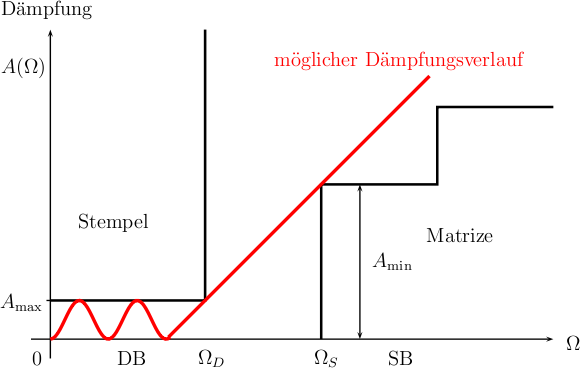
\includegraphics[width=6cm]{./images/filter-toleranzschema.png}}
\end{tabular}

\subsection{Realisation analoger Filter}
\subsubsection{Allgemeines Vorgehen}
\begin{tabular}{p{9cm}|p{9cm}}
    \textbf{UTF} &
    \textbf{LC-Filter} \\
  \hline
    \begin{enumerate}
      \item Toleranzschema (Kap. \ref{toleranzschema}) und Frequenznormierung (Kap. \ref{frequenznormierung})
      \item Äquivalenten normierten TP bestimmen (Kap. \ref{filtertransformation}) (TP)
      \item Tiefpassapproximationsart bestimmen (Kap. \ref{tiefpassapprox}) (TP)
      \item Ordnung für TP bestimmen (Kap. \ref{ordnung}) (TP)
      \item normierte TP UTF bestimmen (Kap. \ref{UTF bestimmen}) (TP)
      \item $\Omega_{3dB}$ bestimmen (Kap. \ref{omega3dB}) (TP)
      \item Rücktransformation und Entnormierung (Kap. \ref{UTF entnormieren} und Kap. \ref{filtertransformation})
    \end{enumerate} &
    \begin{enumerate}
      \item Toleranzschema (Kap. \ref{toleranzschema}) und Frequenznormierung (Kap. \ref{frequenznormierung})
      \item Äquivalenten normierten TP bestimmen (Kap. \ref{filtertransformation}) (TP)
      \item Tiefpassapproximationsart bestimmen (Kap. \ref{tiefpassapprox}) (TP)
      \item Ordnung für TP bestimmen (Kap. \ref{ordnung}) (TP)
      \item Referenzwiderstand bestimmen (Kap. \ref{Rref bestimmen}) (TP)
      \item $L_{FI}$ und $C_{FI}$ bestimmen (Kap. \ref{LC_tabellen}) (TP)
      \item $\Omega_{3dB}$ bestimmen (Kap. \ref{omega3dB}) (TP)
      \item LC Umnormieren (Kap. \ref{LC umnormieren}) (TP)
      \item Filtertransformation (Kap. \ref{LC_transformation})
      \item LC in Impedanz \& Frequenz entnormieren (Kap. \ref{LC entnormieren})
    \end{enumerate}
\end{tabular}


\subsubsection{Frequenznormierung \formelbuch{308}}
\label{frequenznormierung}
\begin{tabular}{ll}
\parbox{6cm}{
	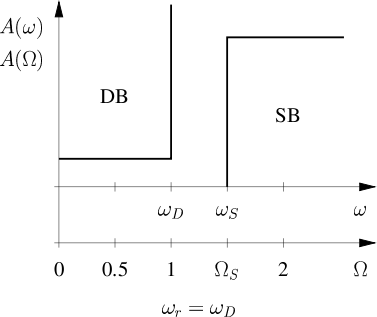
\includegraphics[width=5cm]{./images/filter-freqnormierung.png}}
& \parbox{12cm}{
	\textbf{Normierung} \\
	$\boxed{S=\frac{s}{\omega_{r}} \hspace{2cm} \Omega=\frac{\omega}{\omega_{r}} 
  \hspace{2cm} \sigma'=\frac{\sigma}{\omega_{r}}}$\\ 

	Bei BP \& BS: $\omega_r = \omega_m =\sqrt{\omega_{B1} \omega_{B2}}
	\underbrace{=}_{\text{\tiny{wenn symmetrisch}}} \sqrt{\omega_{S1} \omega_{S2}}$ \\
	
  Bei TP \& HP: $\omega_r = \omega_D$ \\

  \begin{tabular}{ll}
    $\omega_r$: & Referenzfrequenz \\
    $\omega_m$: & Mittenfrequenz \\
    $\omega_D$: & Durchlassfrequenz
  \end{tabular} \\
  Zur Entnormierung wird $\omega_{3db}$ gebraucht, daher sind diese Formeln
	dafür nicht geeignet! \\
	}
\end{tabular}



\subsubsection{Tiefpassapproximationen (TP) \formelbuch{309}}
\label{tiefpassapprox}
\begin{tabular}{|p{9cm}|p{9cm}|}
\hline
\parbox[t]{9cm}{
	\textbf{Butterworth} \formelbuch{310}
	\begin{itemize}
    \item Amplitudengang: Gute Approximation (``maximal flach'', keine Welligkeit)
    \item Allpolfilter: Pole liegen auf dem Einheitskreis mit Abstand $\frac{\pi}{n}$
    \item Gruppenlaufzeit: Leichte Überhöhung bei Grenzfrequenz
    \item Bei $\Omega =1$ hat $|H(j\omega)|$ einen Abfall von 3.01dB
    \item Steilheit im SB: \qquad $-n\cdot 20dB/Dek$
	\end{itemize}
	}
& 
\parbox[t]{9cm}{
	\textbf{Kritisch gedämpftes (Gauss)-Filter} \formelbuch{317}
	\begin{itemize}
    \item Keine Überschwinger bei Impuls- \& Sprungantwort
    \item Kaskadierung von wirkungsfreien identischer Filter 1.Ordnung
    \item Allpolfilter: Pole nur auf negativer $\sigma$-Achse
    \item Gruppen- und Phasenlaufzeit im DB relativ konstant
    \item Bei $\Omega = 1$ hat es eine Dämpfung 3.01dB \\
    \item Steilheit im SB: \qquad $-n\cdot 20dB/Dek$
	\end{itemize}
	} \\
\hline
\parbox[t]{9cm}{
	\textbf{Tschebyscheff I} \formelbuch{321}
	\begin{itemize}
    \item Amplitudengang: Definierte Welligkeit im DB, steiler Übergang
    \item Allpolfilter, wobei alle Pole auf einer Ellipse liegen
    \item Gruppen- und Phasenlaufzeit im DB relativ wellig.
    \item Steilheit im SB: \qquad $-n\cdot 20dB/Dek$
	\end{itemize}
	}
&
 \parbox[t]{9cm}{
	\textbf{Inverser Tschebyscheff  / Tscheby. II} \formelbuch{330}
	\begin{itemize}
    \item Definierte Welligkeit im Sperrbereich
    \item kein Allpolfilter
    \item Gruppen- und Phasenlaufzeit im DB relativ konstant \newline
          (besser als Teschbyscheff I)
	\end{itemize}
	} \\
\hline
\parbox[t]{6cm}{
	\textbf{Cauer (elliptischer Filter)} \formelbuch{333}
	\begin{itemize}
    \item Amplitudengang: Definierte Welligkeit im SB und DB
    \item Steilster Übergang zwischen SB und DB
    \item bei geradem N je N konjugiert komplexe Pol- und Nullstellen
    \item bei ungeradem N 1 reeler Pol und N-1 konjugiert komplexe Pol- Nullstellen
    \item kein Allpolfilter
    \item Gruppen- und Phasenlaufzeit im DB relativ schlecht
    \item kleinste Ordnung
	\end{itemize}
	}
& 
\parbox[t]{6cm}{
	\textbf{Bessel} \formelbuch{339}
	\begin{itemize}
    \item Sehr linearer Phasengang
    \item Flachster Übergang zw. DB und SB im Amplitudengang
    \item ergibt ein Allpolfilter
    \item immer asymptotisch stabil
    \item Gruppen- und Phasenlaufzeit im DB sehr konstant
	\end{itemize}
	} \\
\hline
\end{tabular}
\vfill

\subsubsection{Bestimmung der minimal nötigen Ordnung (TP)}
\label{ordnung}
\begin{tabular}{p{7cm} p{11cm}}
\parbox{6cm}{
	\textbf{Mittels Nomogramm} \\
	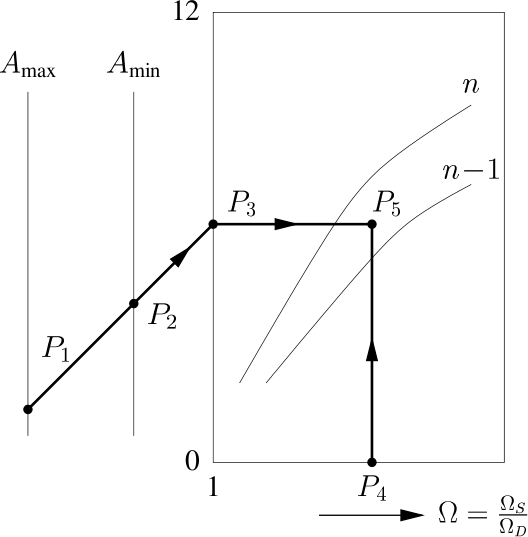
\includegraphics[width=6cm]{./images/filter-nomogramme.png}
	}
& \parbox{12cm}{
	\textbf{Oder mittels Formeln}\\
    
  $n_{\text{Butterworth}} = \left\lceil\frac{\log{\left[\displaystyle\frac{10^{A_{\min}/10}-1}
  {10^{A_{\max}/10}-1}\right]}} {2 \cdot \log{\left(\frac{\Omega_{S}}{\Omega_{D}}\right)}}\right\rceil$
  \formelbuch{316} \\ \\
    
  $n_{\text{Tschebyscheff}_{(\text{I,II})}} = \left\lceil\frac{{\rm Arcosh}
  \sqrt{\displaystyle\frac{10^{A_{\min}/10}-1}{10^{A_{\max}/10}-1}}}
  {{\rm Arcosh}\left({\Omega_{S}/\Omega_{D}}\right)} \right\rceil$
  \formelbuch{327} \\ \\
    
  $n_{\text{Cauer}} = \left\lceil\frac{K\left(\left( \frac{\Omega_D}{\Omega_S}\right)^2\right)
  K\left(1-\frac{10^{A_{\max}/10}-1}{10^{A_{\min}/10}-1}\right) } {K\left(1-\left(\frac{\Omega_D}
  {\Omega_S}\right)^2\right )K\left(\frac{10^{A_{\max}/10}-1}{10^{A_{\min}/10}-1} \right)}\right\rceil,
  \text{mit}\quad
  K(k)=\int_0^{\frac{\pi}{2}}\frac{d\theta}{\sqrt{1-k\sin^2\theta}}$
  \formelbuch{337}\\ \\

	\textbf{Oder mit Matlab}\\
	\texttt{buttord, cheb1ord, cheb2ord, ellipord}	
	}
\end{tabular} \\ \\
\textbf{Grundsätzlich gilt (für gleiche Spezifikationen)} \quad
$n_{\text{Butterworth}}\geq n_{\text{Tschebyscheff}_{(\text{I,II})}}\geq n_{\text{Cauer}}$

\subsubsection{normierte TP UTF bestimmen (TP)}
\label{UTF bestimmen}
Die UTF kann meist aus Tabellen herausgelesen werden und variiert je nach
Filtertyp. Die Entnormierung erfolgt durch Substitution von $S \longrightarrow
\displaystyle\frac{s}{\omega_{\text{3dB}}}$, wobei auch hier
$\omega_{\text{3dB}}$ je nach Filtertyp unterschiedlich berechnet wird.

\label{LC_tabellen}
\renewcommand{\arraystretch}{1.5}
\begin{tabular}{|m{4cm}|m{1.5cm}|m{2.5cm}|m{9.5cm}|}
  \hline
    \textbf{Filtertyp} &
    \textbf{Tabellen auf Seite} &
    \textbf{normiert auf} &
    \textbf{$H(S)$ von TP approximation} \\
  \hline
    Butterworth &
    408 - 409 &
    $\omega_{3dB}$ &
    $ H(S) = \frac{1}{S^n +b_{n-1}S^{n-1}+\ldots+b_2S^2+b_1S+b_0}$ \\
  \hline
    Kritisch-gedämpfte Filter &
    409 - 410 &
    $\omega_{3dB}$ &
    $ H(S) = \frac{K}{S^n +b_{n-1}S^{n-1}+\ldots+b_2S^2+b_1S+b_0} $ \\
  \hline
    Tschebyscheff I &
    412 - 416 &
    $\omega_D$ &
    $ H(S) = \frac{K}{S^n +b_{n-1}S^{n-1}+\ldots+b_2S^2+b_1S+b_0}$ \\
  \hline
    Bessel &
    416 - 418 &
    $\omega_{3dB}$ &
    $ H(S) = \frac{K}{S^n +b_{n-1}S^{n-1}+\ldots+b_2S^2+b_1S+b_0}$ \\
  \hline
    Cauer &
    419 &
    &
    mittels Software \\
  \hline  
\end{tabular}
\renewcommand{\arraystretch}{1}
\begin{tabular}{ll}
  Rippelfehler: & \[e = \sqrt{10^{\frac{A_{max}}{10}}-1}\]
\end{tabular}




\subsubsection{$\Omega_{3dB}$ bestimmen (TP)}
\label{omega3dB}

$\boxed{\Omega_{3dB} \cdot \omega_r = \omega_{3dB}}$

\renewcommand{\arraystretch}{1.5}
\begin{tabular}{|p{6cm}|p{6cm}|p{6cm}|}
\hline
Butterworth \formelbuch{408}
	& Tschebyscheff I \formelbuch{412}
	& Kritisch gedämpfte Filter \formelbuch{409}\\
$\omega_{\text{3dB}}=\underbrace{\sqrt[2n]{\frac{1}{10^{A_{\max}/10}-1}}}_{\Omega_{3dB}}\cdot \omega_{D}$
	&
	$\omega_{\text{3dB}}=\underbrace{\cosh{\left[\left(\frac{1}{n}\right) {\rm
	Arcosh}\left(\frac{1}{e}\right)\right]}}_{\Omega_{3dB}} \cdot \omega_{D}$
	& $\omega_{3\text{dB}}=\frac{\omega_D \cdot{\sqrt{2^{1/n}-1}}
	}{\sqrt{10^{\frac{A_{\text{max}}}{10\cdot n}}-1}}$ \\
\hline
Cauer\formelbuch{419}
	& Bessel \formelbuch{416}
	& \\
Keine Tabelle, \matlab{ellip, ellipap}
	& $\omega_{3\text{dB}}$ aus Abb. 7.112 \formelbuch{417}
	& \\
\hline
\end{tabular}
\renewcommand{\arraystretch}{1}


\subsubsection{Filtertransformationen (TP) \formelbuch{355}}
\label{filtertransformation}
\renewcommand{\arraystretch}{1.5}
\begin{tabular}{|l|l|l|l|}
  \hline
  \multicolumn{2}{|l|}{\textbf{Tiefpass-Hochpass}}
    & \textbf{Tiefpass-Bandpass}
    & \textbf{Tiefpass-Bandsperre} \\ 
  \multicolumn{2}{|l|}{\parbox{6cm}{
    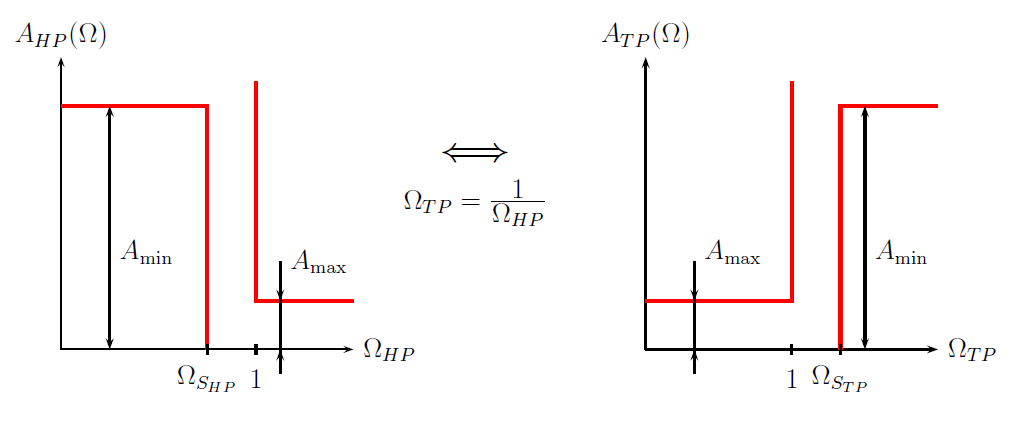
\includegraphics[width=6cm]{./images/filter-transf-tp-hp.png}
    }}
  & \parbox{6cm}{
    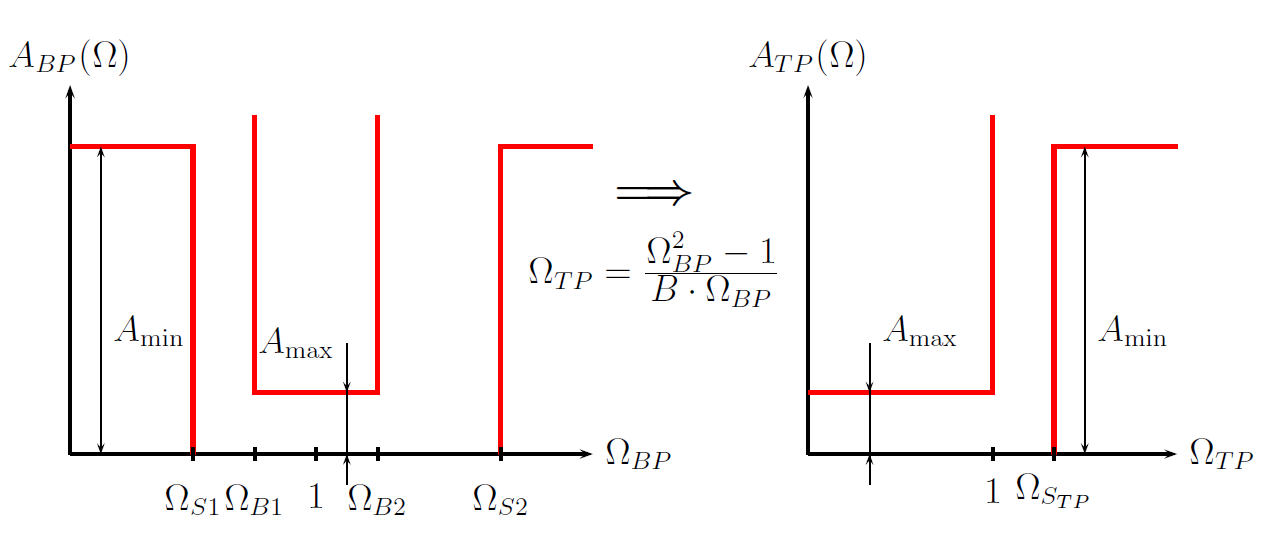
\includegraphics[width=6cm]{./images/filter-transf-tp-bp.png}
    }
  & \parbox{6cm}{
    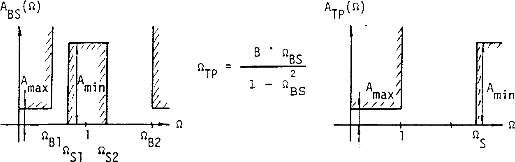
\includegraphics[width=6cm]{./images/filter-transf-tp-bs.png}
    } \\
  \hline \hline
    & \textbf{TP $\Leftrightarrow$ HP} \formelbuch{355} 
    & \textbf{TP $\Leftrightarrow$ BP} \formelbuch{360}
    & \textbf{TP $\Leftrightarrow$ BS} \formelbuch{368} \\
  \hline
  Ordnung: 
    & $n$
    & $2n$
    & $2n$ \\
  \hline
  Ansatz: 
    & $S \longrightarrow \frac{1}{S}$
    & $S \longrightarrow \frac{S^{2}+1}{B\cdot S}$
    & $S \longrightarrow \frac{B\cdot S}{S^{2}+1}$ \\
  \hline
  UTF: 
    &$H_{HP}(S)=H_{TP}\left(\frac{1}{S}\right)$
    & $H_{BP}(S)=H_{TP}\left(\frac{S^{2}+1}{B\cdot S}\right)$
    & $H_{BS}(S)=H_{TP}\left(\frac{B\cdot S}{S^{2}+1}\right)$ \\
  \hline
  Norm. Frequenz: 
    & $\Omega_{S_{TP}}=\frac{1}{\Omega_{S_{HP}}}$
    & $\Omega_{S_{TP}}=\frac{\Omega_{S2}-\Omega_{S1}}{B}=
      \frac{\Omega_{S2}-\Omega_{S1}}{\Omega_{B2}-\Omega_{B1}} =
      \frac{\omega_{S2}-\omega_{S1}}{\omega_{B2}-\omega_{B1}}$
    & $\Omega_{S_{TP}}=\frac{B}{\Omega_{S2}-\Omega_{S1}}=
      \frac{\Omega_{B2}-\Omega_{B1}}{\Omega_{S2}-\Omega_{S1}} =
      \frac{\omega_{B2}-\omega_{B1}}{\omega_{S2}-\omega_{S1}}$ \\
  \hline
  \multicolumn{2}{|l|}{normierte Bandbreite:}
    & \multicolumn{2}{|c|}{$B = \dfrac{\omega_{B2} - \omega_{B1}}{\omega_r} =
      \Omega_{B2}-\Omega_{B1}$} \\
  \hline
  \multicolumn{2}{|l|}{geometrisch-symmetrische BP/BS:}
    & \multicolumn{2}{|c|}{$\Omega_{B1}\Omega_{B2}=\Omega_{S1}\Omega_{S2}=1$}\\
  \hline
  \end{tabular}
  \renewcommand{\arraystretch}{1}
  \\
  
  \textbf{Direkte Substitution}\\
  \renewcommand{\arraystretch}{1.5}
  \begin{tabular}{|lll|}
  \hline
  HP-TP
    & $H_{TP}(S)=\frac{K}{b_{n}S^{n}+b_{n-1}S^{n-1}+...+b_{1}S+b_{0}}$
    & $\longrightarrow
    H_{HP}(S)=\frac{KS^{n}}{b_{0}S^{n}+b_{1}S^{n-1}+...+b_{n-1}S+b_{n}}$\\
  \hline
  BP-TP 1. Ordnung
    & $H_{TP}(S)=\frac{1}{S+a}$
    & $\longrightarrow 
    H_{BP}(S)=H_{TP}\left(\frac{S^{2}+1}{B\cdot S}\right)=\frac{B\cdot
    S}{S^{2}+aB\cdot S+1}$\\
  BP-TP 2. Ordnung
    & $H_{TP}(S)=\frac{1}{S^{2}+aS+b}$
    & $\longrightarrow
    H_{BP}(S)=H_{TP}\left(\frac{S^{2}+1}{B\cdot S}\right)=\frac{B^{2}S^{2}}{S^{4}+aB
    S^{3}+(bB^{2}+2)S^{2}+aB\cdot S+1}$  \\
  \hline 
  BS-TP 1. Ordnung
    & $H_{TP}(S)=\frac{1}{S+a}$
    & $\longrightarrow
    H_{BS}(S)=H_{TP}\left(\frac{B\cdot S}{S^{2}+1}\right)=
    \frac{\frac{1}{a}(S^{2}+1)}{S^{2}+\frac{B}{a}S+1}$ \\
  BS-TP 2. Ordnung
    & $H_{TP}(S)=\frac{1}{S^{2}+aS+b}$ 
    & $\longrightarrow
    H_{BS}(S) = H_{TP}\left(\frac{B\cdot S}{S^{2}+1}\right)=
    \frac{\frac{1}{b}(S^{2}+1)^{2}}{S^{4}+\frac{aB}{b}S^{3}+
    \left(\frac{B^{2}}{b}+2\right)S^{2}+\frac{aB}{b}S+1}$ \\
  \hline
\end{tabular}
\renewcommand{\arraystretch}{1}


\subsubsection{UTF Entnormierung}
\label{UTF entnormieren}
\begin{minipage}[c]{12cm}
  \begin{tabular}{l|l|l|l}
      \textbf{TP}\formelbuch{309} &
      \textbf{HP}\formelbuch{359} &
      \textbf{BP}\formelbuch{365} &
      \textbf{BS}\formelbuch{373} \\
    \hline
      $S=\dfrac{s}{\Omega_{3dB}\cdot \omega_D}$ &
      $S \rightarrow \dfrac{1}{S}$ &
      $S \rightarrow \dfrac{S^2+1}{S\cdot B \cdot \Omega_{3dB}}$ &
      $S \rightarrow \dfrac{S\cdot B \cdot \Omega_{3dB}}{S^2+1}$ \\
      
      &
      $S = \dfrac{s\cdot \Omega_{3dB}}{\omega_D}$ &
      $S = \dfrac{s}{\omega_m}$ &
      $S = \dfrac{s}{\omega_m}$
  \end{tabular}
\end{minipage}
\begin{minipage}[c]{6cm}
  Falls es schon auf $\Omega_D$ (Tschebyscheff I) normiert ist, so gilt $\Omega_{3dB} = 1$
\end{minipage}


\subsubsection{LC-Tiefpass bestimmen (TP) \formelbuch{389/420} }
\label{Rref bestimmen}
\begin{tabular}{ll}
\parbox{10cm}{
	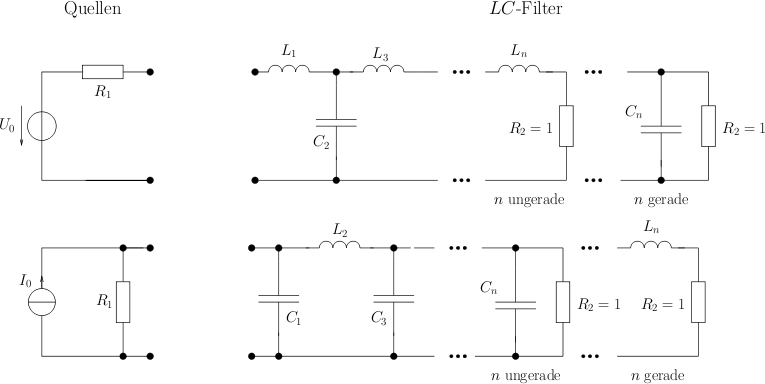
\includegraphics[width=10cm]{./images/filter-lc-realisation.png}
	}
& \parbox{8cm}{
	Die Struktur unterscheidet sich nicht zwischen den Filtertypen.\\
	Es ist zwischen Minimal-C (meistens) und Minimal-L-Netzwerken auszuwählen. \\ \\
  Referenzwiderstand: $\boxed{R_r = R_{\text{Last}}= R_{2_{\text{unnormiert}}}}$
	}
\end{tabular}

\newpage

\subsubsection{LC Tabellenindex (TP)}
\label{LC_tabellen}
\renewcommand{\arraystretch}{1.5}
\begin{tabular}{|p{5.5cm}|p{5.5cm}|p{6cm}|}
\hline
Butterworth \formelbuch{421}
	& Tschebyscheff I \formelbuch{424, 425}
	& Kritisch gedämpfte Filter \formelbuch{423}\\
\hline
Cauer \formelbuch{427, 428}
	& Bessel \formelbuch{422}
	& \\
\hline
\end{tabular}
\renewcommand{\arraystretch}{1}\\
Erläuterungen zu den Tabellen:
	\begin{itemize}
    \item Die Legende oben beschreibt die Stromquellenstruktur, die untere die
      Spannungsquellenstruktur.     
    \item Normierung auf $R_2 = 1$, folglich $R_1 = \frac{R_{\text{Quelle}}}{R_r} = \frac{R_{1_\text{unnormiert}}}{R_r}$
  \end{itemize}

\subsubsection{LC umnormieren (TP)}
\label{LC umnormieren}
$\boxed{L_{FI} = \dfrac{L_{FI3dB}}{\Omega_{3dB}} \qquad
C_{FI} = \dfrac{C_{FI3dB}}{\Omega_{3dB}}}$ \qquad (nicht bei Cauer-Filter)


\begin{tabular}{ll}
\parbox{11.5cm}{
	\subsubsection{Bauteiltransformation zum gewünschten Filter \formelbuch{386}}
  \label{LC_transformation}
	\renewcommand{\arraystretch}{1.5}
	\begin{tabular}{|p{2cm}|p{7.5cm}|}
	\hline
	Tiefpass-Hochpass \formelbuch{386}
		& \parbox{7cm}{
		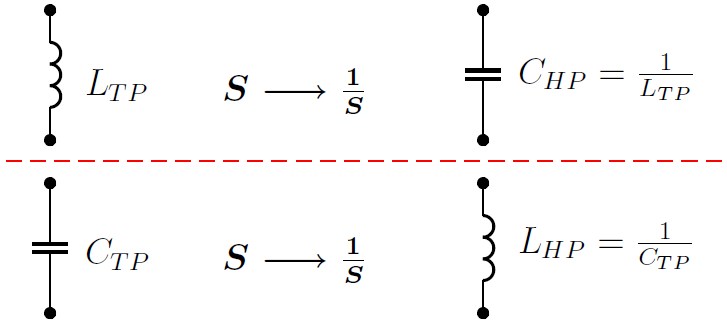
\includegraphics[width=7cm]{./images/filter-bauteile-tp-hp.png}}
		\\
	\hline
	Tiefpass-Bandpass \formelbuch{387}
		& \parbox{7cm}{
		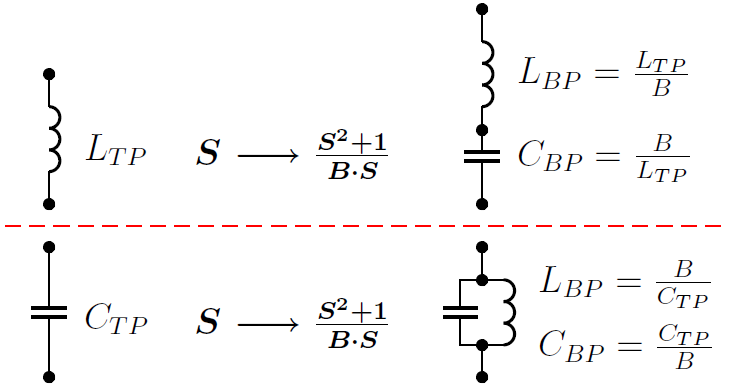
\includegraphics[width=7cm]{./images/filter-bauteile-tp-bp.png}}
		\\
	\hline
	Tiefpass-Bandsperre \formelbuch{388}
		& \parbox{7cm}{
		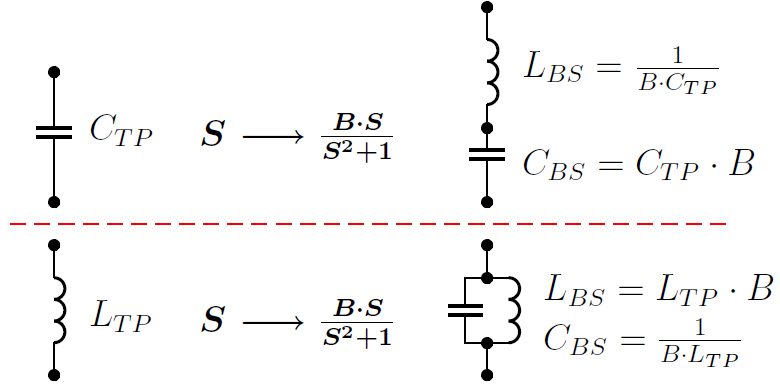
\includegraphics[width=7cm]{./images/filter-bauteile-tp-bs.png}}
		\\
	\hline
	\end{tabular}
	\renewcommand{\arraystretch}{1}
  
  \subsubsection{LC in Impedanz und Frequenz entnormieren\formelbuch{391}}
  \label{LC entnormieren}
  $\boxed{L = L_{FI} \cdot \dfrac{R_r}{\omega_r} \qquad
  C = C_{FI} \cdot \dfrac{1}{R_r \cdot \omega_r}}$
	}
& \parbox{7cm}{
    \subsection{Kaskadierung von Filtern}
      Wenn mehrere Filter kaskadiert werden, ändern sich die Spezifikationen wie in
      folgendem Beispiel:\\
      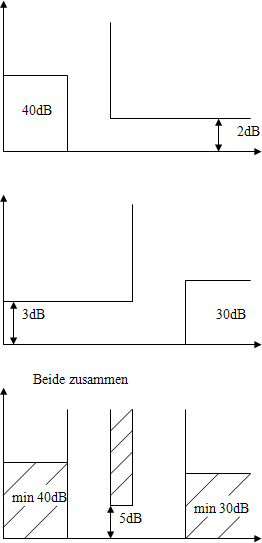
\includegraphics[width=4cm]{./images/filter-kaskadierung.png}
	}
\end{tabular}



\newpage
\subsection{Vergleich der Approximationsarten\formelbuch{344}}
\scriptsize
\begin{center}
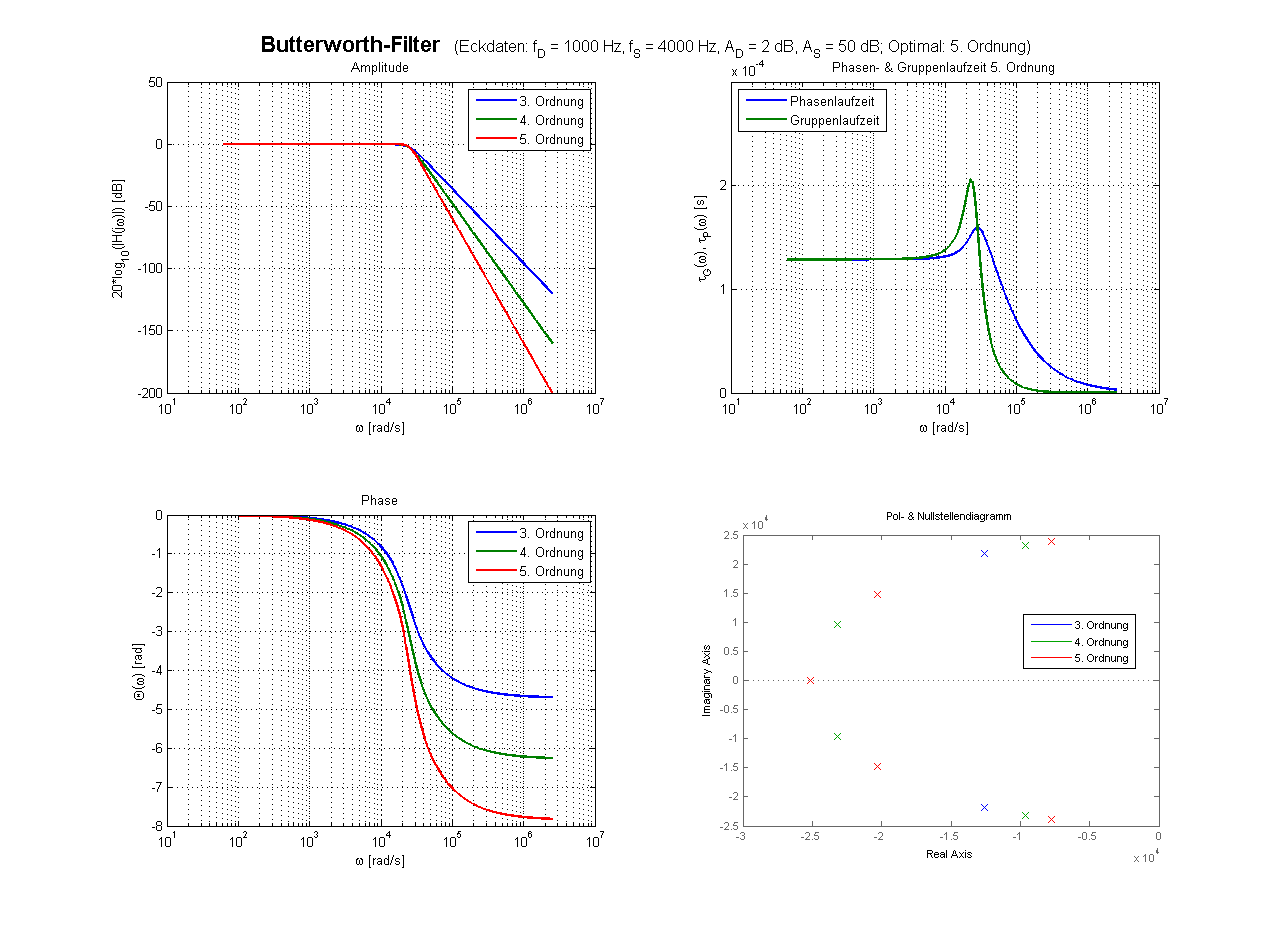
\includegraphics[height=11.5cm]{./images/filter-butterworth.png}
\\Butterworth-Filter mit UTF $H(s) = \frac{1.003e022}{s^5 + 8.133e004 s^4 +
3.307e009 s^3 + 8.312e013 s^2 + 1.291e018 s + 1.003e022}$ 
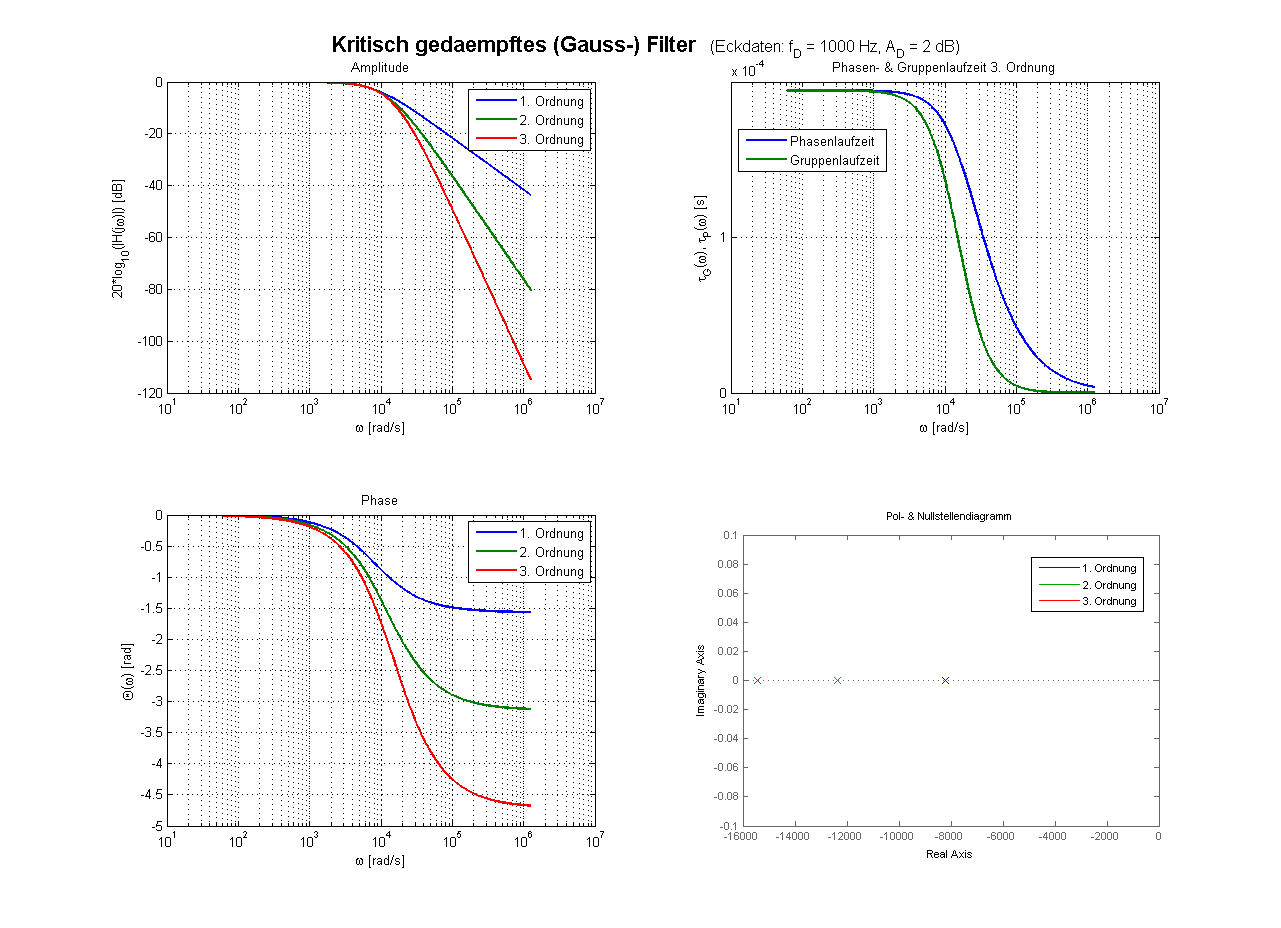
\includegraphics[height=11.5cm]{./images/filter-gauss.png} \\Kritisch gedämpftes
Filter mit UTF $H(s) = \frac{1}{2.724e-013 s^3 + 1.261e-008 s^2 + 0.0001945 s +
1}$ 
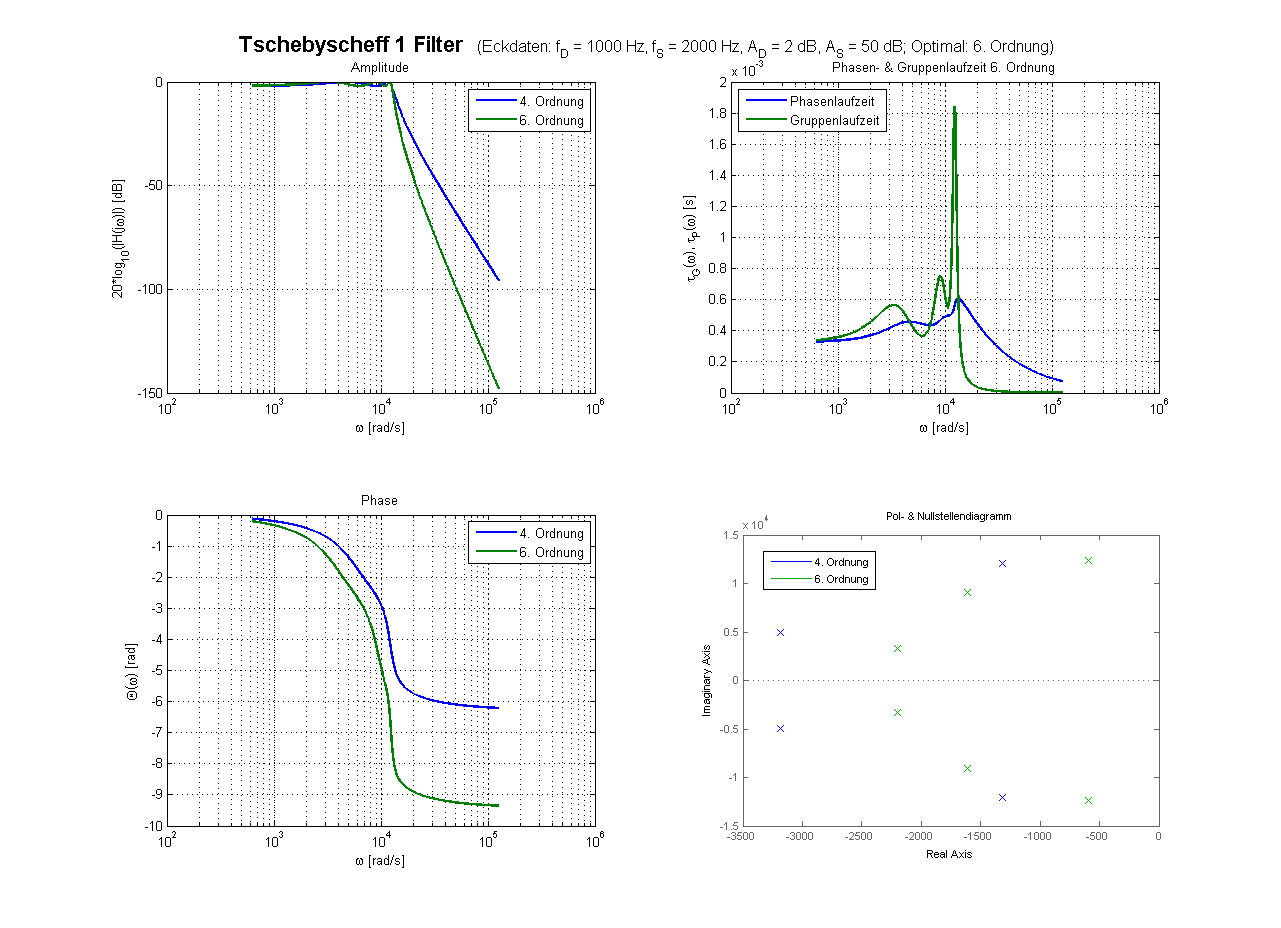
\includegraphics[height=12cm]{./images/filter-tschebyscheff1.png} \\Tschebyscheff-I-Filter mit UTF $H(s)
= \frac{1.609e023}{s^6 + 8812 s^5 + 2.757e008 s^4 + 1.721e012 s^3 + 1.924e016
s^2 + 6.589e019 s + 2.026e023}$ 
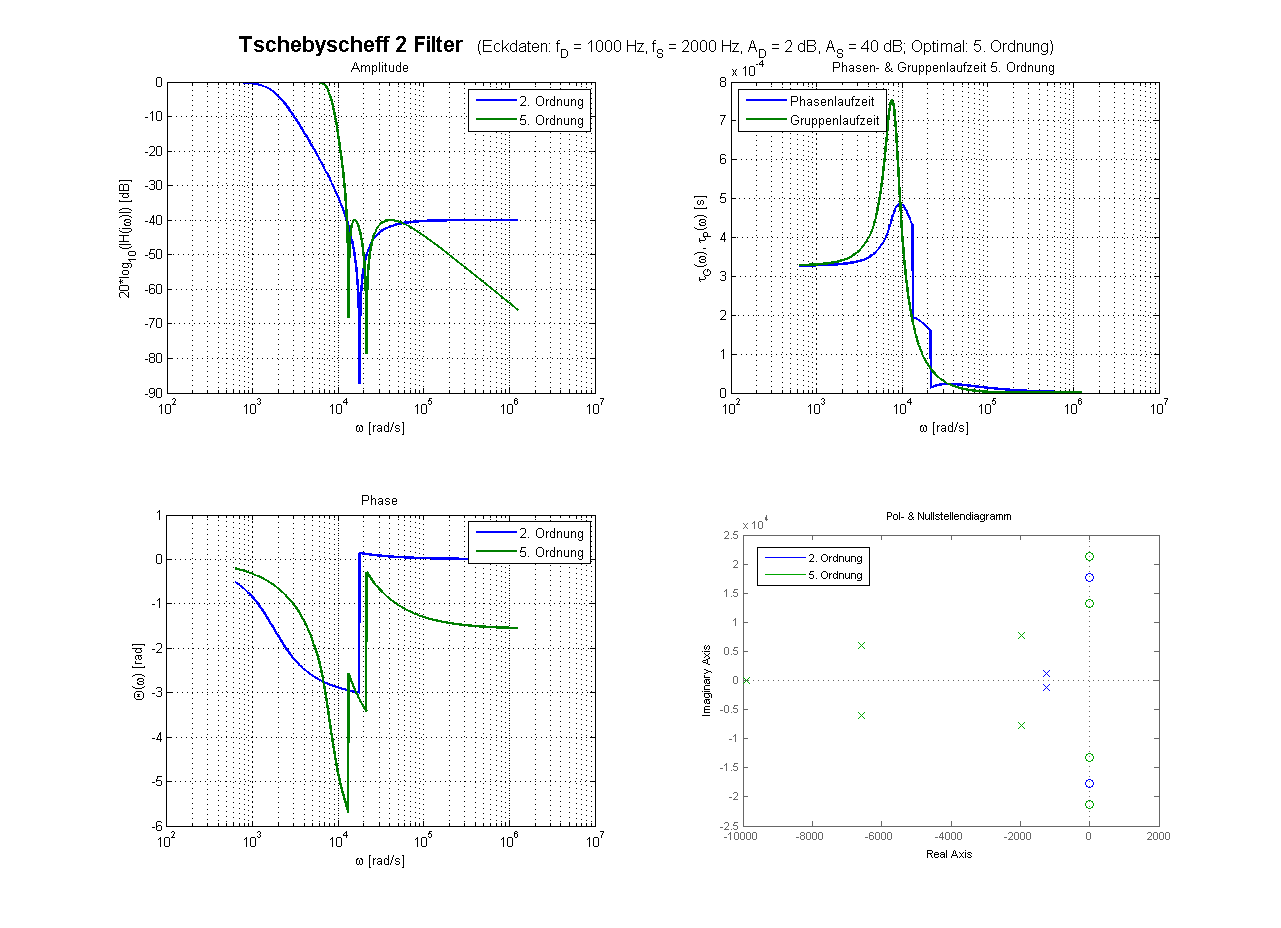
\includegraphics[height=12cm]{./images/filter-tschebyscheff2.png} \\Tschebyscheff-II-Filter mit UTF
$H(s) = \frac{628.3 s^4 + 1.081e-009 s^3 + 3.969e011 s^2 + 1.975 s +
5.014e019}{s^5 + 2.701e004 s^4 + 3.645e008 s^3 + 3.076e012 s^2 + 1.639e016 s + 5.014e019}$
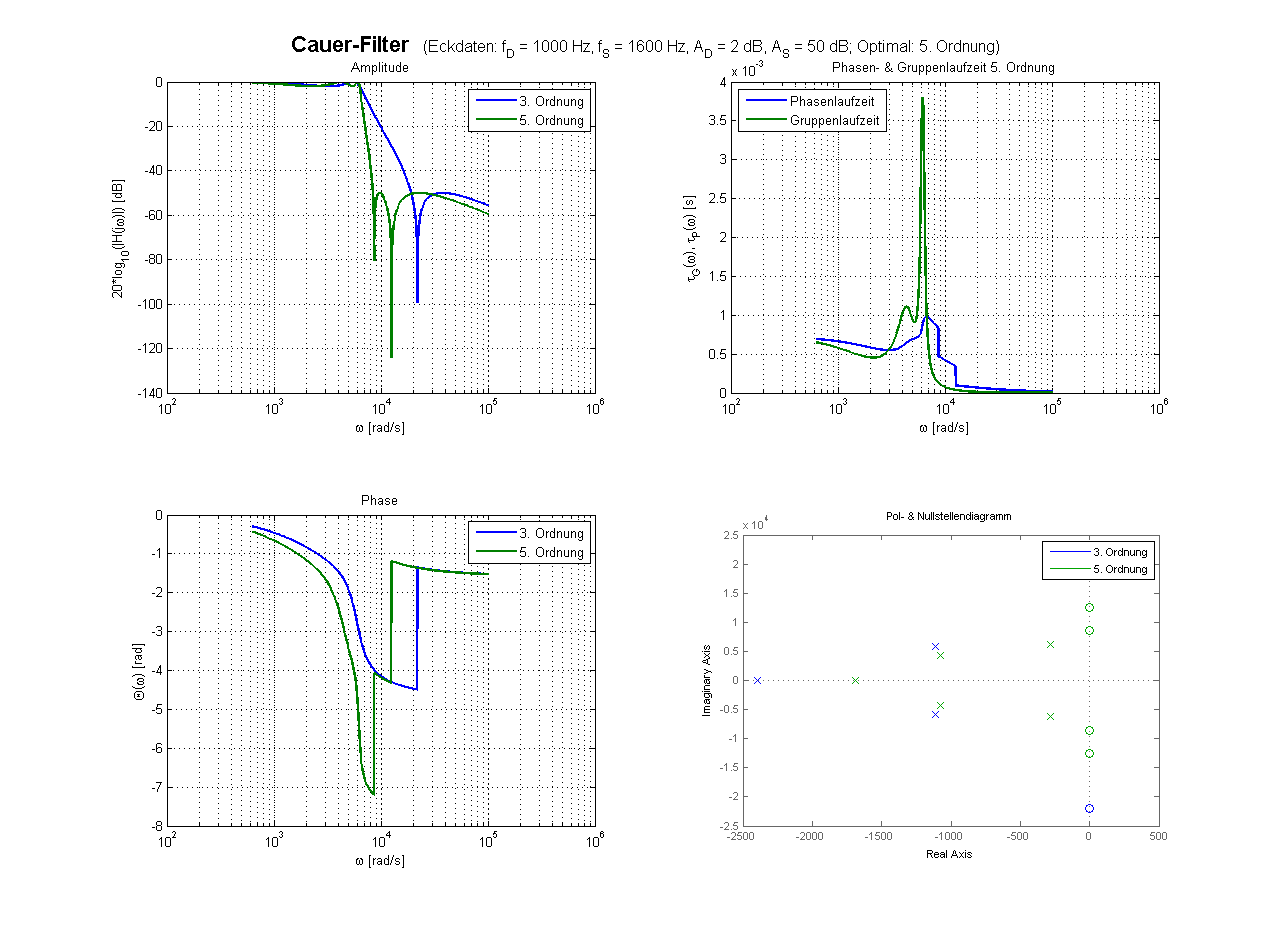
\includegraphics[height=12cm]{./images/filter-cauer.png} \\Cauer-Filter mit UTF
$H(s) = \frac{108.8 s^4 - 6.596e-010 s^3 + 2.538e010 s^2 - 0.08009 s + 1.29e018}{s^5 + 4398 s^4 + 6.408e007 s^3 + 1.939e011 s^2 + 9.227e014 s + 1.29e018}$
\includegraphics[height=12cm]{./images/filter-bessel.png} \\Bessel-Filter mit UTF $H(s) =
 \frac{2.481e011}{s^3 + 1.529e004 s^2 + 9.736e007 s + 2.481e011}$
\end{center}




\end{document}
